% Persistent Anomalies Framework (PAF)
% A Statistical Framework for Operationalizing Human Intuitive Capabilities
% Persistent Anomaly Framework - standalone methods paper
%
% Author: Zach Sparks
% Institution: Arizona State University / Sparks Solutions LLC
% Date: July 2026
%
% Standalone detection-framework paper. v17.1 final public-release edition: fresh per-session committed secrets and full-path randomization.

\documentclass[11pt,letterpaper]{article}

% ============================================================
% PACKAGES
% ============================================================
\usepackage[margin=1in]{geometry}
\usepackage{times}
\usepackage{amsmath,amssymb,amsthm}
\usepackage{algorithm}
\usepackage{algorithmic}
\usepackage{graphicx}
\usepackage{tikz}
\usetikzlibrary{shapes,arrows.meta,positioning,calc,fit,backgrounds,decorations.pathreplacing}
\usepackage{booktabs}
\usepackage{tabularx}
\usepackage{multirow}
\usepackage{caption}
\usepackage{subcaption}
\usepackage{hyperref}
\usepackage{cleveref}
\usepackage{listings}
\usepackage{xcolor}
\usepackage{fancyhdr}
\usepackage{enumitem}
\usepackage{float}

% ============================================================
% STYLE CONFIGURATION
% ============================================================
\hypersetup{
    colorlinks=true,
    linkcolor=black,
    citecolor=black,
    urlcolor=black
}

\pagestyle{fancy}
\fancyhf{}
\fancyhead[R]{\textit{\small Persistent Anomalies: A Statistical Framework}}
\fancyfoot[C]{\thepage}
\renewcommand{\headrulewidth}{0.4pt}
\setlength{\headheight}{14pt}

% Theorem environments
\newtheorem{definition}{Definition}
\newtheorem{theorem}{Theorem}
\newtheorem{proposition}{Proposition}

% Code listing style
\lstset{
    basicstyle=\ttfamily\small,
    keywordstyle=\color{blue!70!black}\bfseries,
    commentstyle=\color{green!50!black}\itshape,
    stringstyle=\color{red!60!black},
    numbers=left,
    numberstyle=\tiny\color{gray},
    numbersep=8pt,
    frame=single,
    framesep=4pt,
    backgroundcolor=\color{gray!5},
    breaklines=true,
    captionpos=b,
    language=Python
}

% TikZ styles
\tikzset{
    block/.style={rectangle, draw, fill=blue!8, text width=6em, text centered, rounded corners, minimum height=3em, font=\small},
    bigblock/.style={rectangle, draw, fill=blue!8, text width=10em, text centered, rounded corners, minimum height=3em, font=\small},
    decision/.style={diamond, draw, fill=orange!15, text width=5em, text centered, aspect=2, inner sep=1pt, font=\small},
    signal/.style={rectangle, draw, fill=green!10, text width=5.5em, text centered, rounded corners, minimum height=2.5em, font=\footnotesize},
    phase/.style={rectangle, draw, fill=blue!15, text width=8em, text centered, rounded corners, minimum height=3.5em, font=\small\bfseries},
    arrow/.style={-{Stealth[length=2.5mm]}, thick},
    layer/.style={rectangle, draw, fill=#1, text width=38em, minimum height=2.2em, font=\small, rounded corners=2pt},
}

\begin{document}

% ============================================================
% TITLE
% ============================================================
\begin{center}
{\LARGE\bfseries Identifying Persistent Anomalies:\\[4pt]
A Statistical Framework for Operationalizing\\[4pt]
Human Intuitive Capabilities}

\vspace{16pt}
{\large Zach Sparks}\\[4pt]
{\small\itshape Sparks Solutions LLC\\
Technological Leadership, BS\\
Interplanetary Initiative, Arizona State University\\
\texttt{zpsparks@asu.edu}}

\vspace{8pt}
{\small July 2026 --- final public-release edition}
\end{center}

\vspace{12pt}

% ============================================================
% ABSTRACT
% ============================================================
\section*{Abstract}
This paper introduces a statistical framework for testing whether human behavioral response streams exhibit persistent dependence on concealed, independently randomized targets in unstructured intuitive tasks. In the primary prospective protocol, an independent key-custody service generates a fresh, non-reusable secret for each response session, commits to that session secret before an unpredictable public-beacon pulse, derives the target key inside a hardware security module, and releases the secret only after that session's response log is cryptographically frozen; a distinct future-key protocol is confined to Appendix~\ref{app:retro}. Such a result is designated here as \textit{persistent target dependence}; the term \textit{persistent anomaly} is reserved as a procedural label for a target-relative effect that survives the registered protocol and an independent replication, not as an ontological claim about a person or mechanism. Rather than relying only on final-answer accuracy, the framework evaluates synchronized gaze, motor or touch trajectory, initial selection, transition, timing, and submitted-response data. The central secondary hypothesis is a two-stage trajectory of target attraction followed by suppression or override. The primary confirmatory endpoint is not cluster resemblance or generic behavioral unusualness, but held-out predictive improvement from conditioning the behavioral stream on the committed target. The complete scoring pipeline is frozen in advance and rerun against the true committed key and a preregistered ensemble of legal reassignment keys generated under the same assignment mechanism. The true-key statistic is evaluated by its legal-key randomization rank, and repeated looks are controlled by ranking a preregistered full-path maximum-excursion statistic across the same exchangeable key ensemble. Clustering and the five noise-as-feature dimensions are retained for screening, mechanism analysis, and post-validation characterization unless explicitly frozen within the primary target-conditioned model. The paper presents a falsifiable measurement architecture rather than evidence that anomalous cognition, retrocausality, or any particular mechanism exists. Consent, pseudonymization, independent oversight, and auditable governance are specified throughout.

\medskip
\noindent\textbf{Keywords:} persistent target dependence, concealed-target testing, randomization inference, conditional independence, behavioral telemetry, empirical mutual information, anomaly detection, intuitive cognition, unstructured testing

% ============================================================
% 1. INTRODUCTION
% ============================================================
\section{Introduction}

\subsection{The Third Analytical Modality}

The intelligence community has historically relied on two primary analytical modalities: signals intelligence (SIGINT) derived from technical collection systems, and human intelligence (HUMINT) derived from interpersonal networks and observation. A possible third modality, intuitive cognition, refers here to putative individual differences in pattern detection, anticipatory judgment, and below-threshold synthesis, a capacity that has been explored intermittently but never systematically operationalized within a rigorous empirical framework.

Project Stargate (1972--1995) and its sibling programs investigated such capabilities for intelligence applications and were ultimately terminated amid inconsistent replication and methodological criticism (Section~2). A persistent, low-amplitude, distributed signal, if present, would be poorly matched to the single-session, performance-on-demand scoring those programs employed. The present framework adopts a measurement design suited to that signal profile.

\subsection{Measurement Approach}
\label{sec:measurement}

The framework sets aside the contested question of whether anomalous cognition exists and the unfalsifiable question of subjective experience, and evaluates instead whether a subject's behavioral output carries statistical structure with respect to hidden ground truth.

Reports of exceptional intuition are common in everyday and professional decision contexts. Many individuals report a sincere subjective sensation of knowing that a response was correct. Neuroimaging and behavioral measures may eventually help distinguish subjective confidence, motor commitment, and final response selection, since the sensation of knowing, the motor pathway actually taken, and the submitted answer need not coincide.

This creates a three-way dissociation that prior programs never resolved:

\begin{enumerate}[nosep]
    \item \textbf{Subjective experience:} The individual reports a sensation of knowing. \textit{Measurable as self-report, but not independently diagnostic of target access.}
    \item \textbf{Decision pathway:} Motor cortex commits to a response, potentially overriding the intuitive signal. \textit{Measurable via behavioral monitoring.}
    \item \textbf{Statistical output:} Across hundreds of trials, the behavioral stream carries non-random structure with respect to hidden targets. \textit{Measurable and testable.}
\end{enumerate}

The measurement architecture remains mechanism-agnostic. For participant $i$, item $j$, and session $t$, let $\mathbf{B}_{ijt}$ denote the preregistered behavioral observation vector in target-agnostic coordinates (for example raw gaze, motor or touch, initial selection, reversal, latency, and final response); let $A^*_{jt}$ denote the concealed target identity; let $L_{ajt}$ denote the displayed location of option $a$; and let $Z_{ajt}$ denote target-independent visual or aesthetic properties of option $a$. The conventional covariate vector $\mathbf{X}_{ijt}$ may contain device, session, prior response, layout, the complete set $\{L_{ajt},Z_{ajt}\}_{a=1}^{M}$ represented symmetrically, latency range, and calibration quality. No component of $\mathbf{X}$, its preprocessing, or its feature construction may depend on which option is designated by a candidate key. Target-relative quantities, including the location occupied by the candidate target, are constructed exclusively inside the target-conditioned branch and reconstructed separately for every legal reassignment key. The governing confirmatory hypothesis is
\begin{equation}
H_0:\ \mathbf{B}_{ijt} \perp A^*_{jt}\mid\mathbf{X}_{ijt}
\qquad\text{versus}\qquad
H_1:\ \mathbf{B}_{ijt} \not\!\perp A^*_{jt}\mid\mathbf{X}_{ijt}.
\label{eq:core}
\end{equation}
The realized target vector is fixed after commitment, but its target labels vary across trials. Empirical target--behavior dependence, including empirical mutual information, can therefore be estimated from the observed trial-level pairs $(A^*_{jt},\mathbf{B}_{ijt})$. Inferential calibration is supplied by legal reassignments drawn from the same preregistered key-generation mechanism, so that the committed key is compared with keys that are exchangeable with it under $H_0$.

Mutual information remains a useful descriptive quantity because target coupling may appear as attraction toward or avoidance of the target. To leading order in a small per-item coupling $\delta$, information is approximately symmetric in sign because $I\propto\delta^2$ near chance. The symmetry is not exact for $M>2$ options: avoidance distributes probability across $M-1$ non-target options and therefore has a lower attainable maximum than attraction. Final-answer accuracy can discard this structure, but a below-chance final score is not itself evidence; it becomes informative only when the complete frozen pipeline shows target-specific dependence relative to legal key reassignments.

The primary empirical objective is to determine whether target conditioning improves held-out prediction of the behavioral stream beyond a target-independent model and whether that improvement persists across independently randomized sessions. The framework integrates four components: (1) concealed targets generated through a public committed procedure; (2) multimodal behavioral monitoring; (3) full-pipeline randomization inference and sequential error control; and (4) secondary noise-as-feature and trajectory analyses for mechanism characterization. Bayesian quantities may be reported as model-based summaries, but the confirmatory decision is design-based and target-conditioned.

\subsection{Scope and Applications}

The immediate scope is methodological: testing concealed-target dependence under controlled randomization. Components of the telemetry and validation architecture could later be adapted to study conventional intuition, forecasting, or expert decision-making, but those applications require separate tasks with real predictive structure, independent validation, and domain-specific ethics review.

\subsection{Methodological Context}

Across large populations performing forced-choice tasks, some above-chance outliers are expected on distributional grounds alone, and repeated testing is required to distinguish transient sampling extremes from reproducible target-specific structure: in any sufficiently large sample, some individuals will deviate from chance in a given session by ordinary sampling variation, and persistence across independently randomized sessions separates a reproducible pattern from a transient extreme. Such outliers are a near-certainty; the motivating question of this work is whether the reproducible, target-specific ones can be rigorously identified and characterized, regardless of mechanism.

This paper develops a detection framework for a contentious empirical domain using formal hypotheses, adversarial controls, and statistical signal detection. This design has two consequences:

\begin{enumerate}[nosep]
    \item \textbf{Scientific:} If target dependence is observed, the protocol separates the statistical finding from competing explanations such as ordinary bias, unconscious inference, or a nonstandard mechanism.
    \item \textbf{Operational:} Intelligence applications require capability, not explanation. The question ``can this individual provide statistically significant information about hidden states?'' is operationally relevant.
\end{enumerate}

The contribution is a measurement architecture for testing the anomaly hypothesis.

% ============================================================
% FIGURE 1: Three-Phase Pipeline Overview
% ============================================================
\begin{figure}[t]
\centering
\resizebox{\textwidth}{!}{%
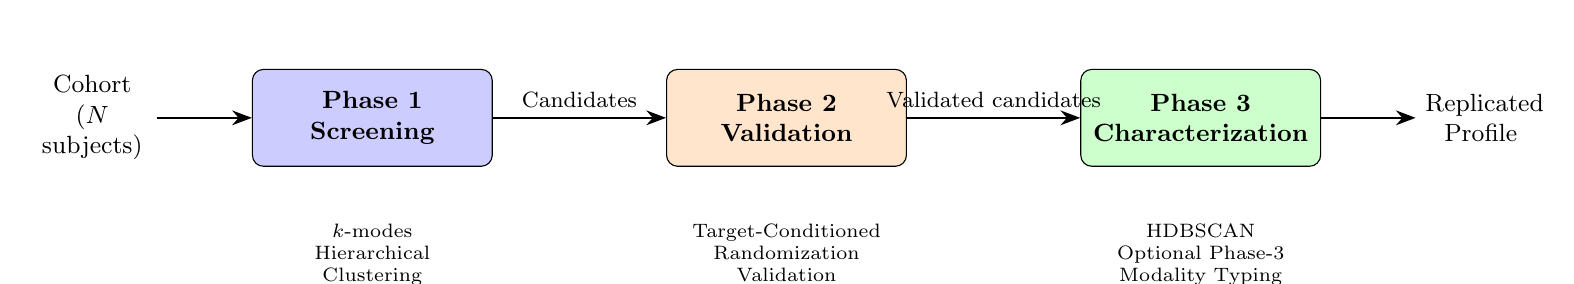
\begin{tikzpicture}[node distance=1.8cm]
    % Phases
    \node[phase, fill=blue!20] (p1) {Phase 1\\Screening};
    \node[phase, fill=orange!20, right=2.2cm of p1] (p2) {Phase 2\\Validation};
    \node[phase, fill=green!20, right=2.2cm of p2] (p3) {Phase 3\\Characterization};
    
    % Arrows
    \draw[arrow] (p1) -- node[above, font=\footnotesize] {Candidates} (p2);
    \draw[arrow] (p2) -- node[above, font=\footnotesize] {Validated candidates} (p3);
    
    % Methods below
    \node[below=0.6cm of p1, text width=7em, text centered, font=\scriptsize] {$k$-modes\\Hierarchical\\Clustering};
    \node[below=0.6cm of p2, text width=7em, text centered, font=\scriptsize] {Target-Conditioned\\Randomization\\Validation};
    \node[below=0.6cm of p3, text width=7em, text centered, font=\scriptsize] {HDBSCAN\\Optional Phase-3\\Modality Typing};
    
    % Input/Output
    \node[left=1.2cm of p1, font=\small, text width=4em, align=center] (input) {Cohort\\($N$ subjects)};
    \node[right=1.2cm of p3, font=\small, text width=4em, align=center] (output) {Replicated\\Profile};
    \draw[arrow] (input) -- (p1);
    \draw[arrow] (p3) -- (output);
\end{tikzpicture}%
}
\caption{Three-phase persistent target-dependence identification pipeline. Phase 1 screens cohorts via clustering to identify candidates. Phase 2 tests target dependence by comparing the committed-key evidence path with the same frozen pipeline evaluated on legal reassignment keys, using a full-path randomization rank that includes every registered look. Phase 3 characterizes replicated target-dependent cases via density-based clustering and supervised classification.}
\label{fig:pipeline}
\end{figure}

\subsection{What This Paper Does and Does Not Claim}

No empirical validation is reported here; the framework awaits data (Section~\ref{sec:roadmap}). It does not claim that anomalous cognition has been demonstrated, that any individual possesses it, or that any mechanism has been established.

The claim is falsifiable and specific. If an anomalous signal of the low-amplitude, distributed kind described above exists, episodic performance scored by final-answer accuracy in single sessions is structurally mismatched to it and would miss it. The framework instead targets reproducible, target-specific mutual information distributed across the behavioral stream, tested longitudinally and under adversarial controls. If the signal is absent, the committed-key statistic should be unexceptional within the legal-key randomization distribution, and apparent structure should fail the calibrated sequential test.

% ============================================================
% 2. BACKGROUND
% ============================================================
\section{Background \& Related Work}

Cold War concern over Soviet parapsychology research led the U.S.\ intelligence community to investigate anomalous cognition through classified programs, most extensively Project Stargate, conducted under the Defense Intelligence Agency primarily at Stanford Research Institute under Harold Puthoff and Russell Targ \cite{puthoff1976,targ1977}. Declassified records document hundreds of operational remote-viewing missions \cite{mcmoneagle1997,smith2005}, and a portion of the laboratory record was assessed as statistically significant \cite{utts1996}; the program was nonetheless terminated in 1995 after an American Institutes for Research evaluation questioned operational utility amid inconsistent replication and methodological criticism \cite{air1995}. For the present framework the operative lesson is methodological: Stargate-era evaluation emphasized episodic performance on structured tasks rather than longitudinal target-coupling, and its designs left open the leakage, judging, and analytic-flexibility channels that the controls of Sections~\ref{sec:committed-key} and~\ref{sec:lockbox} are built to close.

The framework's statistical logic has precedent in conventional domains. In financial markets, persistent risk-adjusted excess return is treated as evidence of analytical capability rather than luck, distinguishable through longitudinal tracking \cite{fama2010}; in clinical medicine, diagnostic accuracy that persistently exceeds base rates identifies expert pattern recognition not captured by explicit decision rules \cite{norman2017}. Persistence distinguishes candidate capability from chance, provided target-specificity controls rule out fixed bias. Institutional acceptance of the narrower premise, that exceptional human judgment exists in the population, can be tracked longitudinally, and carries operational value, is demonstrated by IARPA's forecasting programs and the superforecaster literature \cite{tetlock2015}; the persistent anomaly framework adapts that longitudinal-performance logic from structured forecasting to unstructured hidden-target assessment. Independently, quantum cognition has emerged as a formal modeling language for judgment phenomena that resist classical probability description \cite{busemeyer2012,pothos2013}; the framework's statistics do not depend on that formalism, and it is not developed further here.

% ============================================================
% 3. METHODOLOGY
% ============================================================
\section{Methodology}

\subsection{Conceptual Framework}

The identification of persistent target dependence proceeds through three phases (Figure~\ref{fig:pipeline}): screening, validation, and characterization. Each phase employs distinct task designs and statistical methods calibrated to the specific identification objective.

\begin{definition}[Persistent Target Dependence and Persistent Anomaly]
Let $\mathcal{P}$ denote a fully registered protocol and let $T_i(\mathbf{A})$ denote its frozen target-conditioned confirmatory statistic for participant $i$ evaluated under key $\mathbf{A}$. A participant exhibits \textit{validated target dependence under $\mathcal{P}$} when the committed-key statistic crosses the preregistered sequential randomization boundary on held-out sessions while the identical pipeline remains calibrated under legal reassignment keys. The term \textit{persistent anomaly} is a procedural designation applied only after the target-relative result is reproduced in an independent preregistered replication. Before replication, the participant is a candidate with a protocol-specific finding, not a person assigned a stable trait or status.
\end{definition}

\begin{definition}[Persistent Target-Dependence Hypothesis]
The core hypothesis is that a small subset of participants may exhibit target-conditioned behavioral structure that is:
\begin{enumerate}[nosep]
    \item consistent across independently randomized, temporally separated sessions;
    \item robust to task reformulation and target-position randomization;
    \item significant under the full-pipeline legal-key randomization test;
    \item not attributable to the preregistered conventional predictors $\mathbf{X}$; and
    \item independently replicable before any persistent designation is applied.
\end{enumerate}
\end{definition}

\subsection{Unstructured Task Design}

To minimize cognitive priming, participants complete tasks with minimal context and no performance feedback. The canonical example is a \textit{blank response matrix}: participants are presented with an answer sheet containing $N$ items with $M$ response options each, instructed only to ``respond to each item.'' No questions are provided. Responses therefore provide a minimally cued behavioral stream shaped by internal processes, guessing, and response habits.

Although tasks appear unstructured to the participant, each item has a designated target fixed by the registered assignment mechanism. This concealed target transforms the protocol from measuring generic deviation from uniform responding into testing target-relative dependence. The participant experiences an unstructured task; the sealed scoring system contains the target key, which is inaccessible to participants, administrators, and analysts during administration.

Additional task variants include abstract pattern completion (geometric sequences with a single correct solution not deducible from context), temporal ordering of randomized event descriptions (with known chronology), and forced-choice color or symbol selection (with hidden target). Tasks satisfy four design criteria:

\medskip
\noindent\textbf{Criterion 1 (Null baseline):} Under the null hypothesis $H_0$ (random responding), the expected response distribution is known and uniform:
\begin{equation}
P(\mathbf{r} \mid H_0) = \prod_{j=1}^{N} \frac{1}{M} = M^{-N}
\end{equation}
This expression defines the idealized independent-uniform null for the canonical task; downstream validation replaces it with calibrated transition nulls wherever serial dependence or response bias is empirically present (Section~\ref{sec:lr}).

\noindent\textbf{Criterion 2 (Minimal priming):} Task presentation minimizes information that could guide responses through conventional reasoning.

\noindent\textbf{Criterion 3 (Iterative stability):} Tasks can be reformulated across sessions without altering the underlying statistical structure, enabling longitudinal comparison.

\noindent\textbf{Criterion 4 (Hidden ground truth):} Each item has a definite designated target $a_j^*$ fixed by the registered assignment mechanism of Section~\ref{sec:committed-key} but inaccessible to the participant through conventional means. This enables directional deviation analysis:
\begin{equation}
\delta_i^{(t)} = \frac{1}{N} \sum_{j=1}^{N} \mathbb{1}[r_{ij}^{(t)} = a_j^*] - \frac{1}{M}
\label{eq:directional}
\end{equation}
The signed quantity $\delta_i$ records the \textit{direction} of target coupling: $\delta_i > 0$ indicates attraction toward the target, $\delta_i < 0$ indicates systematic avoidance of it. Consistent with the central premise (Section~1.2), the detection statistic is the \textit{magnitude} of coupling, $|\delta_i|$, or, more generally, the empirical mutual information $I(\mathbf{R}_i; \mathbf{A}^*)$; the sign of $\delta_i$ is retained only to assign a sub-type (attractor or suppressor) once an anomaly has been detected. A subject whose responses are reliably anti-correlated with the target carries comparable information to a correlated subject in the small-coupling regime; at large couplings the avoidance signal is bounded below the attraction signal for $M > 2$ (Section~\ref{sec:measurement}), so the sign also constrains the maximum attainable magnitude.

\subsection{Competence-Free Items and the Intellect Dissociation}
\label{sec:nonsense}

A persistent above- or below-chance coupling on a semantically meaningful item, one with a defensible correct answer reachable by knowledge or reasoning, is confounded. It may reflect intuitive access to the target, but it may equally reflect intellect: a subject who reasons well, recognizes patterns, or knows the relevant fact will couple to the answer through entirely conventional means. The statistical deviation may be real, but its source remains ambiguous.

The framework resolves this ambiguity by including a class of \textit{competence-free} items, for which conventional reasoning is structurally excluded. A competence-free item pairs a prompt that admits no reasoned answer with a fixed but arbitrary target drawn from the response options. To sustain engagement, such items are presented as genuine forced-choice questions rather than as self-evident nonsense: a non-linguistic or abstract stimulus, for example a colored field or an abstract glyph, is shown, followed by a set of response options of which one is committed in advance as the target. The respondent encounters a forced-choice item with a definite designated target that cannot be reached by reasoning, rather than a prompt whose absurdity signals that no response is intended. A non-linguistic prompt also carries far less recoverable semantic or phonetic structure than a nonsense sentence, reducing the surface available for inadvertent experimenter-introduced structure. The response options are generated under the orthogonal multi-source protocol of Section~\ref{sec:orthogonal} and the target among them is assigned by the committed-secret/public-beacon mechanism of Section~\ref{sec:committed-key}, so that ordinary option-preference biases, such as a pull toward a particular number or position, are not aligned with the committed target and are further removed by the aesthetic-baseline residualization of Section~\ref{sec:aesthetic}. Because the prompt is designed to contain no recoverable structure, ordinary knowledge or reasoning should not systematically move a subject's responses toward or away from the committed target. The space of explanations is thereby narrowed: either the response stream is independent of the committed target, which is the null, or an apparent coupling must survive controls for leakage, bias, and key-generation artifacts, and, if the construction succeeds, competence becomes a less plausible explanation for any residual coupling.

This yields a diagnostic contrast across item types that is stronger than either type alone. An effect driven by intellect should appear on sensible items and vanish on competence-free items, where there is nothing to reason toward. An effect of the kind the framework is designed to detect should appear on the competence-free items, where it constitutes the clean measurement, and may additionally appear on sensible items through the confounded channel. The pattern of presence and absence across the two item classes is itself the falsifiable claim, and it allows the framework to distinguish anomalous coupling from ordinary cognitive competence without resolving the question of mechanism.

The dissociation holds only under a strict condition on the target. If the competence-free target carried any recoverable structure, if the experimenter's choice of which option to designate were predictable, habitual, or otherwise modelable, then a subject could couple to the experimenter's key-generation process rather than to the target, reintroducing a conventional channel under the guise of anomalous detection. The inference becomes interpretable only when the target is generated by a process neither the experimenter nor the subject can predict or influence, and committed before responses are collected. The construction that satisfies this requirement is specified in Section~\ref{sec:committed-key}.

\subsection{Orthogonal Item-Generation and Aesthetic-Decoupling Controls}
\label{sec:orthogonal}

The competence-free dissociation requires more than a committed answer key. It requires that the competence-free items themselves carry no experimenter-introduced structure, since an item whose prompt, options, or target reflects the designer's aesthetic or linguistic habits is no longer genuinely structureless, and a subject could couple to that residual structure through ordinary means. The prompt $P$, answer-option set $O$, and question-to-target mapping $M$ are independently randomized by construction using separated entropy sources and pipelines. The design seeks, but does not assume or prove, negligible dependence:
\begin{equation}
I(P;O) \approx 0,\quad I(P;M) \approx 0,\quad I(O;M) \approx 0,
\label{eq:orthog}
\end{equation}
and, more strongly, the joint generation factorizes,
\begin{equation}
P(P,O,M) = P(P)\,P(O)\,P(M),
\label{eq:factorize}
\end{equation}
with the generated corpus audited for detectable dependence using preregistered tests. Failure to detect dependence does not prove independence; it establishes only that no dependence exceeding the audit sensitivity was observed. A concrete realization distributes generation across three decoupled sources: a prompt generator that produces semantically empty stimuli, whether non-linguistic fields such as colors or abstract glyphs or strings composed from pre-vetted syntactic components, under one entropy source; an option-pool generator that produces abstract answer choices with no semantic relationship to the prompt under a second, independent source; and a combinatorial mapper that fixes presentation order and the designated target under the committed-secret/public-beacon mechanism of Section~\ref{sec:committed-key}. Separating the sources removes a major common-cause channel, but does not by itself prove that generation artifacts are absent. The corpus audit, aesthetic controls, legal-key randomization test, and independent replication jointly determine whether a detected association survives those explanations.

\subsection{Behavioral Monitoring Layer}
\label{sec:behavioral}

The final submitted response captures only the endpoint of the decision process. The framework augments response data with continuous behavioral monitoring that captures pre-conscious and pre-submission dynamics (Table~\ref{tab:behavioral}).

In computer-administered protocols, four synchronized data streams are recorded where the device and consent conditions permit:

\begin{enumerate}[nosep]
    \item \textbf{Motor or touch trajectory:} On desktop systems, mouse position $\mathbf{m}(t) = (x(t), y(t))$ sampled at $\geq 60$\,Hz \cite{freeman2011}, including velocity $\dot{\mathbf{m}}(t)$, acceleration $\ddot{\mathbf{m}}(t)$, and hover duration. On touch devices, the corresponding stream includes touch-down location, drag path, pressure where exposed by the device, correction gestures, and time from first contact to commitment.
    \item \textbf{Attention or gaze trajectory:} With separate informed consent, front-facing-camera gaze estimation records target-relative fixation order, dwell proportion, revisitation, disengagement, and the temporal relationship between visual attention and touch or click behavior. Consumer-camera gaze is treated as a noisy behavioral sensor, not as a clinical eye tracker, and is calibrated per device and participant.
    \item \textbf{Selection history:} The complete sequence of selections and deselections $\{(s_k, t_k)\}_{k=1}^{K_j}$ for each item $j$, including the initial selection $s_1$, any changes, and the final submission $s_{K_j}$.
    \item \textbf{Timing profile:} Response latency $\Delta t_j$ per item, inter-item interval, total session duration, and the timing offsets among gaze, movement, initial selection, reversal, and submission.
\end{enumerate}

\paragraph{Target-relative gaze and suppression signature.}
Let $D_{ij}(a)$ denote the proportion of valid gaze dwell assigned to option $a$ for participant $i$ on item $j$. The target-attention advantage is
\begin{equation}
G_i = \frac{1}{N}\sum_{j=1}^{N}\left[D_{ij}(a_j^*) - \frac{1}{M-1}\sum_{a\neq a_j^*}D_{ij}(a)\right].
\label{eq:gazeadvantage}
\end{equation}
Because option locations are independently randomized, a fixed preference for a screen region follows the location rather than the candidate target and is removed by participant-, device-, and position-specific controls. The gaze-suppression event for item $j$ is the ordered trajectory
\begin{equation}
\text{neutral scan} \rightarrow \text{target fixation} \rightarrow \text{target dwell or revisit} \rightarrow \text{disengagement} \rightarrow \text{non-target commitment}.
\label{eq:gazesuppression}
\end{equation}
Its evidentiary statistic is the excess frequency of that trajectory relative to matched trials with the same interface layout, option-location set, latency range, and calibration quality. Candidate-target location is derived only within the target-conditioned statistic and is recomputed for every legal key. Gaze contributes evidence only when it tracks the concealed target as the target moves across randomized option locations and survives the legal-key reference ensemble; raw looking time, a preferred corner, or systematic calibration drift is not evidence of target coupling.

The behavioral layer accounts for the conscious override phenomenon: a subject may initially select the target in a pattern consistent with below-threshold attraction, and then change to a non-target response because ``I can't possibly know this.'' This override pattern produces a specific signature:

\begin{definition}[Override Index]
For participant $i$ on item $j$, let $s_1^{(j)}$ denote the initial selection and $s_K^{(j)}$ the final submission. The override index is:
\begin{equation}
O_i = \frac{1}{N} \sum_{j=1}^{N} \mathbb{1}[s_1^{(j)} = a_j^* \;\wedge\; s_K^{(j)} \neq a_j^*]
\label{eq:override}
\end{equation}
Under the null hypothesis (random initial and final selections), $O_i$ has a nonzero chance baseline of $\frac{1}{M}\left(1 - \frac{1}{M}\right)$ rather than zero, so a raw count of correct-then-reversed transitions is uninformative on its own. The chance baseline is moreover only a first approximation: initial and final selections are not independent, since reversals depend on item difficulty, response latency, expressed confidence, and interface condition. The appropriate null is a \textit{transition model} estimated from the subject's own non-target items and from matched control items,
\begin{equation}
P\big(s_K = b \mid s_1 = a,\, \text{item},\, \text{latency},\, \text{confidence},\, \text{condition}\big),
\label{eq:transition}
\end{equation}
which captures the subject's baseline propensity to revise any initial selection under given conditions. The anomalous feature is the \textit{excess} of target-correlated reversals relative to this matched transition baseline: the degree to which initially-correct selections are reversed \textit{beyond} what the subject's general revision behavior predicts, and specifically toward the committed target rather than uniformly. A participant who reverses initially-correct selections at a rate significantly exceeding their matched baseline, and does so specifically with respect to the target, exhibits the suppression signature: the intuitive signal is being detected and then overridden. Consistent with Section~1.2, the same transition machinery detects the mirror case, in which a subject reverses initially-incorrect selections \textit{toward} the target beyond baseline; both are target-coupled transition structure and differ only in sign.

The transition baseline of Eq.~\ref{eq:transition} is conditioned in part on item difficulty, but competence-free items (Section~\ref{sec:nonsense}) carry no objective difficulty metric, and a subject's propensity to revise an initial selection on a competence-free item need not match their revision behavior on a sensible item where they can second-guess their own reasoning. A baseline trained on sensible items would therefore mis-predict the reversal rate on competence-free items. The competence-free override baseline is trained exclusively on other competence-free negative-control items, so that the excess-reversal statistic on a competence-free target is compared only against the subject's revision behavior on items of the same structurally meaningless class.

This mechanism yields a falsifiable within-subject manipulation. If the override account is correct, the measured deviation should increase as conscious deliberation is suppressed, for example under speeded, offhand, or non-deliberate responding, and decrease under conditions that encourage deliberate attention to the item. The prediction is directional and testable within a single subject: target coupling is expected to be strongest when the pre-deliberative response is captured before the conscious override can act, and weakest when the subject reasons about the item. This manipulation also discriminates between two competing explanations for any observed coupling. A genuine pre-conscious coupling should strengthen under deliberation suppression, whereas a motor-timing or device-coupling artifact should be indifferent to whether the subject is deliberating, since the artifact does not depend on the cognitive pathway. A deliberation-dependence test is included as a design element rather than a post hoc observation.
\end{definition}

The five layers of the decision process produce a signal hierarchy (Table~\ref{tab:behavioral}). Historical final-answer scoring measured only the last layer. The framework measures layers 2 through 5: attention, motor commitment, selection transition, and final response. Layer 1, subjective sensation, may motivate the hypothesis but is not treated as diagnostic evidence.

\begin{table}[h]
\centering
\caption{Five-layer signal hierarchy. The framework targets attention, motor, and selection-transition layers, where weak target-relative structure may be detectable in aggregate before it is lost at final submission.}
\label{tab:behavioral}
\small
\begin{tabular}{@{}clllc@{}}
\toprule
& \textbf{Layer} & \textbf{What Happens} & \textbf{Expected Form} & \textbf{Measurable?} \\
\midrule
1 & Phenomenological & ``I knew it'' sensation & Subjective report & Self-report only \\
2 & Attention/Gaze & Early fixation or dwell on $a_j^*$ & Frequent but noisy & In aggregate \\
3 & Motor/Touch & Trajectory biased toward $a_j^*$ & Frequent but weak & In aggregate \\
4 & Selection & Target-first, then reversal & Intermittent & Per-trial \\
5 & Response & Correct or target-avoiding submission & Lowest-amplitude endpoint & Conventional \\
\bottomrule
\end{tabular}
\end{table}

The behavioral monitoring layer expands the noise-as-feature analysis (Section~\ref{sec:naf}). Gaze and motor trajectories that consistently approach the target before disengaging contribute to temporal asymmetry (N1). Override patterns that suppress target-directed attention, movement, or initial selections produce the directional bias captured by N2. Variance in suppression frequency across cognitive-load conditions maps to context-modulated variance (N3). Cross-device replication and target-position randomization further distinguish target-relative structure from interface or calibration artifacts. The behavioral layer may therefore recover target-coupled structure that final-answer scoring would discard.

\subsection{Embedded Deployment and Answer-Pattern Encoding}

The standalone screening session described in Section~3.2 is the canonical protocol, but the framework may gain statistical power and scalability when embedded within standardized assessments that subjects are already taking. Voluntary military aptitude batteries such as the ASVAB, officer selection examinations, and military college entrance tests provide natural embedding vehicles, since subjects are cognitively engaged, test-taking infrastructure is established, and behavioral monitoring via computer-administered testing is standard. Because these are consented selection instruments, they are an appropriate setting for embedding, but any such use would require explicit informed consent for secondary anomaly scoring, beyond the ordinary consent for cognitive assessment.

\subsubsection{Passive Embedding}

In the simplest configuration, a small number of embedded hidden-target items ($n_{\text{psi}}$) are distributed among the standard test items ($n_{\text{test}}$). Each hidden-target item presents a conventional-looking question whose standard correct answer is known, but whose \textit{hidden target} answer is drawn from a separate key $\mathbf{A}^*_{\text{psi}}$. The subscript $\psi$ denotes the hidden-target scoring key associated with the anomalous-cognition hypothesis; it does not assume that the hypothesis is true. Within a consented hidden-target protocol, the subject answers normally and the sealed scoring system later scores against both keys after the response log is frozen.

This approach has limited statistical power because $n_{\text{psi}}$ must remain small relative to $n_{\text{test}}$ to avoid detection. With a typical $n_{\text{psi}} = 10$--$20$ items per test and $M = 4$ options, the per-session trial count is low.

\subsubsection{Answer-Pattern Encoding}
\label{sec:ape}

A more powerful approach encodes the psi signal not in individual items but in the sequential pattern of responses across standard test items. The subject answers ordinary test questions with ordinary correct answers. The psi signal is embedded in the \textit{differential accuracy} on designated versus non-designated item pairs.

The experimenter partitions all adjacent item pairs into two sets: \textit{designated} pairs $\mathcal{P}_D$ (fraction $\phi$ of all pairs, typically $\phi \approx 0.3$) and \textit{control} pairs $\mathcal{P}_C$. This partition constitutes the psi key $\mathbf{A}^*_{\text{psi}}$. The subject has no knowledge of the partition.

\begin{definition}[Pair Accuracy]
For participant $i$, the pair accuracy on designated and control pairs is:
\begin{align}
\hat{p}_D(i) &= \frac{1}{|\mathcal{P}_D|} \sum_{(j,j+1) \in \mathcal{P}_D} \mathbb{1}[(r_j, r_{j+1}) = (a_j, a_{j+1})] \label{eq:pd} \\
\hat{p}_C(i) &= \frac{1}{|\mathcal{P}_C|} \sum_{(j,j+1) \in \mathcal{P}_C} \mathbb{1}[(r_j, r_{j+1}) = (a_j, a_{j+1})] \label{eq:pc}
\end{align}
The psi test statistic is the differential pair accuracy:
\begin{equation}
\Delta_i = \hat{p}_D(i) - \hat{p}_C(i)
\label{eq:pattern}
\end{equation}
\end{definition}

Under the null hypothesis (no psi influence on designated pairs), pair accuracy is uniform across the partition and $\mathbb{E}[\Delta_i \mid H_0] = 0$, regardless of the subject's overall test performance. A high-performing student scores well on \textit{both} designated and control pairs equally; a low-performing student scores poorly on both. The differential $\Delta_i$ reduces overall ability confounds, since it compares designated and control pairs within the same subject.

The null variance is:
\begin{equation}
\text{Var}(\Delta_i \mid H_0) = p_i(1-p_i)\left(\frac{1}{|\mathcal{P}_D|} + \frac{1}{|\mathcal{P}_C|}\right) + \text{Cov}_{\text{overlap}}
\label{eq:pairnull}
\end{equation}
where $p_i = p_j \cdot p_{j+1}$ is the subject's expected pair accuracy estimated from overall test performance. Adjacent pairs $(j, j+1)$ and $(j+1, j+2)$ share an item, so their indicators are positively correlated and $\text{Cov}_{\text{overlap}} > 0$; the independent-binomial term alone understates the null variance and is anti-conservative. A valid test therefore either restricts to non-overlapping pairs, for which the covariance term vanishes (a 100-item test yields 50 non-overlapping pairs), or estimates the full variance by the Markov-surrogate null introduced below. Worked illustratively on non-overlapping pairs for a subject at 70\% item accuracy, the null standard deviation is of order $0.1$ and the corresponding significant deviation is of order $\Delta_i \gtrsim 0.2$; the overlapping-pair figures should not be used for inference.

The independent-product form $p_i = p_j \cdot p_{j+1}$ is, however, only a first approximation, because human response streams carry local sequential dependencies, including alternation bias, gambler's-fallacy guessing, and fatigue-induced error bursting. If a subject's idiosyncratic local rhythm, for example a habitual answer change every third item, happens to align with the designated partition $\mathcal{P}_D$, then $\Delta_i$ will deviate from zero for an entirely conventional reason. The null model is therefore upgraded from independent Bernoulli trials to a first-order Markov chain with transition matrix $\hat{P}(R_{t} \mid R_{t-1})$, and the expected designated-pair accuracy and its variance are computed under that fitted transition model before the designated subset is evaluated. Fitting the transition matrix on the full stream, including the designated pairs, partially absorbs any genuine signal into the null and therefore biases the test toward zero; this is conservative. Where the loss of power matters, the transition model is instead fitted on the control pairs only, leaving the designated subset out of the null estimation. The designated-versus-control differential is then assessed against the subject-specific Markov null rather than against an independence assumption that local response habits would violate.

In principle no additional items are required, though ethical deployment would require explicit consent. A 200-item test produces 199 overlapping adjacent pairs, or 100 non-overlapping adjacent pairs if independence between pair units is required. Combined with triplet and higher-order patterns, the effective trial count per session is increased modestly; because overlapping patterns are statistically dependent, $n_{\text{eff}}$ grows substantially more slowly than the raw pattern count, and the Markov-surrogate null governs validity rather than the nominal count.

\subsubsection{Scale and Longitudinal Feasibility}
Large cohorts can estimate population-level effects more precisely, but pooled power does not confer reliable per-person classification. Population screening must account for the number of individuals tested, the assumed prevalence, and positive predictive value, while individual validation depends on each participant's own longitudinal evidence. The framework therefore requires end-to-end simulation of familywise error or false-discovery control before any large-cohort study.

Weak effects may require many sessions per participant. A recurring research protocol can accumulate those sessions more feasibly than a one-time study, but participation must be voluntary and separated from employment, promotion, assignment, discipline, education, or benefits. The present manuscript proposes a statistical testbed, not an institutional readiness or personnel-selection program.

\subsubsection{Dual-Use Considerations at Scale}

The same mathematics could in principle be applied, without consent, to data individuals produced for other purposes, including standardized test archives and institutional records. For a dual-use method, open development under governance is safer than concealment. Secondary anomaly scoring constitutes a new use requiring explicit informed consent; identification must trigger no recruitment, surveillance, or compulsory status (Section~\ref{sec:ethics}); and the method, its assumptions, controls, and limitations are published openly so that consent, auditability, and governance structures can be established before any deployment rather than after.

\subsection{The Committed Key: Eliminating Experimenter Influence}
\label{sec:committed-key}

Every target in this framework is interpretable only if its assignment is independent of participant behavior and beyond discretionary experimenter control. The primary prospective concealed-target protocol and the future-key protocol of Appendix~\ref{app:retro} use the same commitment principles but different beacon timing.

\paragraph{Primary prospective concealed-target protocol.}
The item set, target-derivation algorithm, beacon schedule, legal assignment space, primary endpoint, model class, and analysis code are preregistered and cryptographically hashed before enrollment. For each response session $t$, an independent key-custody service generates a fresh uniformly random 256-bit secret $S_t$ inside a hardware security module (HSM), publishes a binding commitment to $S_t$ before that session's unpredictable beacon epoch, and retains the secret without participant, administrator, investigator, or confirmatory-analyst access. The selected public-beacon pulse $B_t$ occurs after this commitment but \emph{before} session $t$. The HSM combines the fresh committed session secret, the locked protocol hash, and $B_t$ to derive that session's prospective target key and legal reassignment keys. The realized targets exist during responding but remain inaccessible within the sealed scoring service. After the behavioral log, timestamps, software version, and completeness metadata for session $t$ are cryptographically frozen, the custodian releases $S_t$ so that the commitment and every derived key can be independently verified. A committed secret is never reused across sessions; each independently randomized session has its own commitment, beacon pulse, target-key ensemble, and post-freeze secret release.

\paragraph{Distinct future-key protocol.}
Appendix~\ref{app:retro} specifies a different temporal intervention. There the response dataset is collected and cryptographically frozen first; only afterward does the preregistered beacon pulse occur and generate a target that did not exist during responding. Because the responses are already immutable, temporary target secrecy is not required to prevent participant leakage in that design. Results from the future-key design are not pooled with, or described as, evidence from the primary prospective concealed-target experiment.

Both designs require:
\begin{enumerate}[nosep]
\item \textbf{Pre-registration.} The protocol, item set, target-derivation algorithm, legal assignment space, key timing, primary endpoint, and analysis code are registered and hashed before the relevant commitment point.
\item \textbf{Public randomness.} The target is derived from a preregistered pulse of a public randomness beacon generated outside the laboratory. In the prospective protocol the pulse follows the secret commitment and precedes response collection; in Appendix~\ref{app:retro} it follows the frozen response dataset.
\item \textbf{Committed prospective secret.} Before each prospective session $t$, an independent HSM generates a fresh $S_t\leftarrow\{0,1\}^{256}$ uniformly and publishes a commitment $C_{S_t}$ before that session's beacon pulse. The secret is inaccessible outside the custody service until that session's response log is frozen, and $S_t$ is never reused.
\item \textbf{Deterministic, domain-separated derivation.} The committed secret, protocol hash, beacon value, legal-key index, item index, and rejection counter are mapped to targets by a published algorithm with no discretionary re-rolling or post hoc selection.
\item \textbf{Sealed custody and verifiable release.} The HSM audit log demonstrates that neither $S_t$ nor the realized session target key was revealed before that session's log freeze. Release of $S_t$ afterward permits public verification of the commitment and the complete session key ensemble.
\item \textbf{Non-selective epoch rule.} Every successfully committed session secret and preregistered beacon epoch must be used for its designated session. HSM failure, inability to derive or release $S_t$, premature access, or any aborted session is retained in the public protocol ledger as a failure and may not be silently replaced by a new secret, beacon epoch, or target realization.
\item \textbf{Identical legal-key inference.} The committed key and all legal reassignment keys are generated from the same preregistered assignment mechanism and evaluated by the identical complete scoring pipeline.
\end{enumerate}

This construction addresses both discretion and concealment. Commitment before the unpredictable beacon prevents the custodian from choosing $S_t$ in response to the realized session beacon; temporary secrecy prevents participants or investigators from publicly reconstructing the prospective key during administration; deterministic release permits independent verification after log freeze; and the non-selective epoch rule prevents favorable-key retention through silent aborts. These controls do not establish that the item corpus is artifact-free, so corpus audits, legal-key randomization, and independent replication remain necessary.

A concrete realization makes the prospective procedure auditable end to end. Let
\begin{equation}
P_H=\operatorname{SHA256}(\text{Protocol})
\end{equation}
be the hash of the locked protocol. Before the preregistered beacon epoch for session $t$, the HSM generates a fresh uniformly random secret $S_t$ and publishes the domain-separated commitment
\begin{equation}
C_{S_t}=\operatorname{SHA256}\!\left(\text{``PAF-secret-v1''}\,\|\,P_H\,\|\,t\,\|\,S_t\right).
\label{eq:secretcommit}
\end{equation}
After the session-$t$ beacon publishes $B_t$ but before response collection begins, the HSM derives one seed for the committed key ($k=0$) and $K$ seeds for legal reassignment keys ($k=1,\ldots,K$):
\begin{equation}
Q_{tk}=\operatorname{HMAC\text{-}SHA256}\!\left(S_t,\,P_H\,\|\,t\,\|\,B_t\,\|\,\text{``Key''}\,\|\,k\right).
\label{eq:keyseed}
\end{equation}
For item $j$ and rejection counter $c=0,1,\ldots$, define
\begin{equation}
H_{tjkc}=\operatorname{HMAC\text{-}SHA256}\!\left(Q_{tk},\,\text{``Item''}\,\|\,j\,\|\,\text{``Ctr''}\,\|\,c\right),
\end{equation}
and interpret the digest as an unsigned integer $U_{tjkc}\in\{0,\ldots,2^{256}-1\}$. To avoid modulo bias for arbitrary $M$, let
\begin{equation}
L_M=\left\lfloor\frac{2^{256}}{M}\right\rfloor M.
\end{equation}
The service selects the first counter $c^*$ for which $U_{tjkc^*}<L_M$ and sets
\begin{equation}
a_{tjk}=1+\big(U_{tjkc^*}\bmod M\big).
\label{eq:targetindex}
\end{equation}
This rejection-sampling rule is exactly uniform over the $M$ options; direct modulo reduction is used only when $M$ divides $2^{256}$. For session $t$, the committed target key is $\mathbf{A}^{*}_t=\mathbf{A}^{(0)}_t$, and $\mathbf{A}^{(1)}_t,\ldots,\mathbf{A}^{(K)}_t$ form the verifiable legal-key ensemble. After the session log is frozen, release of $S_t$ allows any auditor to verify Eq.~\ref{eq:secretcommit}, reproduce every $Q_{tk}$, and reconstruct every item target for that session. The next session begins with a newly generated $S_{t+1}$ and a new commitment; no disclosed secret is ever carried forward. The future-key appendix uses the separately registered post-response beacon timing described there; it must not be represented as the prospective construction above.

\medskip
The iterative nature of the testing protocol is essential. Single-session deviations, regardless of magnitude, are insufficient for a persistent designation. The session budget is determined prospectively by end-to-end power simulations under the registered target-conditioned statistic; weak or intermittent effects may require tens of independently randomized sessions.

\subsection{The Noise-as-Feature Paradigm}
\label{sec:naf}

Conventional psychometric screening treats noise as error, variance to be averaged out so a clean signal can emerge. The persistent anomaly framework instead models the temporal and directional dependencies within the residual distribution, evaluating whether a subject produces structured deviations that are statistically non-random across time, context, and task. The protocol analyzes structure in error rather than accuracy alone, and this move distinguishes it from both classical psychometric assessment and prior anomalous cognition research programs.

If anomalous cognition exists in the form targeted here, it may manifest below conscious control, intermittently, context-sensitively, and buried in stochastic processes. It need not present as a stable channel; it would surface as bias, drift, timing anomalies, clustering, or anticipation effects embedded in otherwise noisy outputs. Treating noise as a feature follows directly from the hypothesis being tested.

The framework analyzes noise along five dimensions (Figure~\ref{fig:naf}):

\begin{enumerate}[nosep]
    \item \textbf{Temporal asymmetry (N1):} Does deviation cluster \textit{before} stimuli, not just after?
    \item \textbf{Error directionality (N2):} Are mistakes biased in a consistent direction rather than symmetrically random?
    \item \textbf{Context-modulated variance (N3):} Does variance change systematically with emotional, cognitive, or environmental load?
    \item \textbf{Cross-task coherence (N4):} Do unrelated tasks show correlated anomaly signatures?
    \item \textbf{Heavy-tail distributions (N5):} Are tails heavier than Gaussian expectation? Are there excess coincidences?
\end{enumerate}

These noise parameters apply standard signal-processing primitives adapted from fault detection, signals intelligence, network anomaly detection, and early-warning systems, and they require no commitment to anomalous cognition.

The noise-as-feature paradigm maintains the separation between screening and validation (Section~3.1): screening identifies who is statistically unusual; validation establishes why. Many prior programs blurred these steps, making interpretation difficult. The framework keeps them separate, allowing identification of outliers without requiring mechanistic explanation, an approach compatible with high-stakes evaluation standards.

Treating large deviation in either direction as candidate signal widens the space of false positives, and two distinct failure modes must be separated from candidate target coupling. The first is the chance extreme: in a large cohort, some null responders will deviate far from chance on a single session purely by sampling. This failure mode is reduced by \textit{persistence}. Extreme single-session scores produced by chance regress toward the mean on retest, whereas genuine coupling does not; and the larger the per-session item count, the more decisively this filter operates, because the probability of reaching an extreme by chance falls sharply with the number of items. With hundreds of items, the probability of a chance responder reaching the extreme tail can become vanishingly small under the specified null, so a deviation that recurs across reformulated sessions is correspondingly difficult to attribute to sampling. The second failure mode is the mundane fixed bias: a subject who is reliably ``wrong'' for a conventional reason, misreading the format, inverting a scale, a stable response habit, will also persist across sessions. This failure mode is reduced by \textit{target specificity} and negative-control keys. A subject with a fixed response bias deviates relative to every key, including the negative-control keys, because their behavior is a property of the subject and not of the target; a candidate target-coupled anomaly should deviate relative to the committed target specifically and sit near chance against the control keys. Anomaly status therefore requires both conditions jointly: persistence across reformulated sessions, which suppresses chance extremes, and specificity against negative-control keys (Section~\ref{sec:committed-key}), which tests against fixed response biases. Either criterion alone is insufficient; their conjunction supports an inference of reproducible, target-specific coupling to ground truth.

% ============================================================
% FIGURE: Noise-as-Feature Architecture
% ============================================================
\begin{figure}[t]
\centering
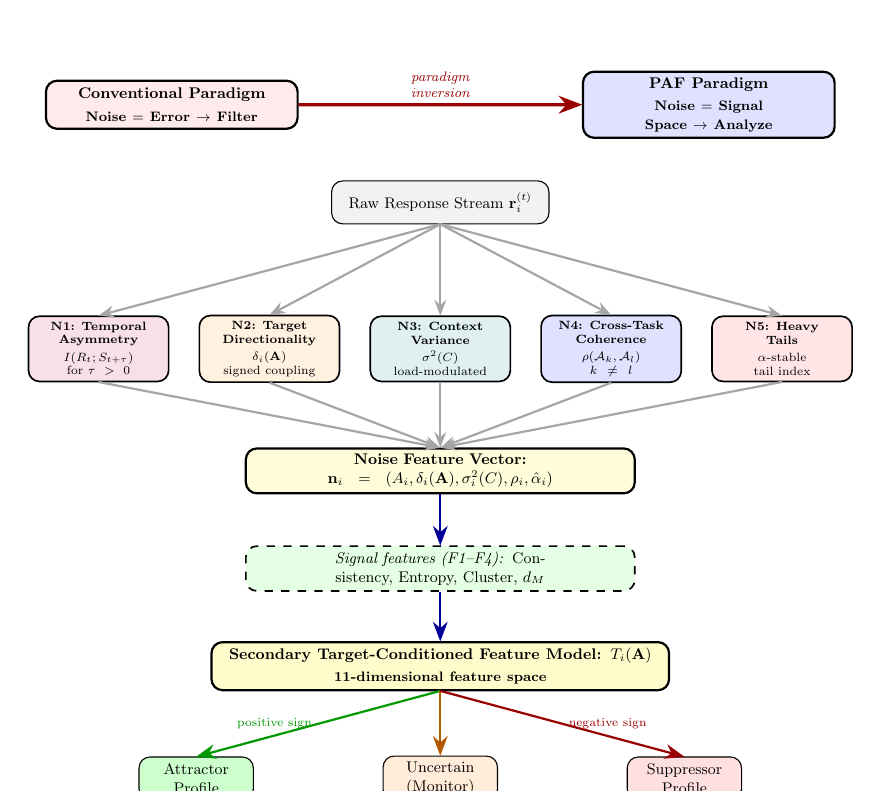
\begin{tikzpicture}[scale=0.62, every node/.style={transform shape}]

% === TOP: The Paradigm Inversion ===
\node[rectangle, draw, fill=red!8, text width=14em, text centered, rounded corners, 
      minimum height=2.8em, font=\small\bfseries, line width=0.8pt] 
      (conventional) at (-5.5, 8) {Conventional Paradigm\\[2pt]\footnotesize Noise $=$ Error $\to$ Filter};

\node[rectangle, draw, fill=blue!12, text width=14em, text centered, rounded corners, 
      minimum height=2.8em, font=\small\bfseries, line width=0.8pt] 
      (inverted) at (5.5, 8) {PAF Paradigm\\[2pt]\footnotesize Noise $=$ Signal Space $\to$ Analyze};

\draw[-{Stealth[length=3mm]}, very thick, red!60!black] (conventional) -- 
    node[above, font=\footnotesize\itshape, text width=8em, align=center] {paradigm\\inversion} (inverted);

% === RAW INPUT ===
\node[rectangle, draw, fill=gray!10, text width=12em, text centered, rounded corners,
      minimum height=2.5em, font=\small] 
      (raw) at (0, 6) {Raw Response Stream $\mathbf{r}_i^{(t)}$};

% === FIVE NOISE DIMENSIONS ===
\tikzset{
    nfdim/.style={rectangle, draw, fill=#1, text width=7.5em, text centered, 
                  rounded corners, minimum height=3.8em, font=\scriptsize, 
                  line width=0.6pt}
}

\node[nfdim=purple!12] (ta) at (-7, 3) {\textbf{N1: Temporal}\\\textbf{Asymmetry}\\[2pt]$I(R_t; S_{t+\tau})$\\for $\tau > 0$};
\node[nfdim=orange!12] (ed) at (-3.5, 3) {\textbf{N2: Target}\\\textbf{Directionality}\\[2pt]$\delta_i(\mathbf{A})$\\signed coupling};
\node[nfdim=teal!12]   (cv) at (0, 3) {\textbf{N3: Context}\\\textbf{Variance}\\[2pt]$\sigma^2(C)$\\load-modulated};
\node[nfdim=blue!12]   (ct) at (3.5, 3) {\textbf{N4: Cross-Task}\\\textbf{Coherence}\\[2pt]$\rho(\mathcal{A}_k, \mathcal{A}_l)$\\$k \neq l$};
\node[nfdim=red!10]    (ht) at (7, 3) {\textbf{N5: Heavy}\\\textbf{Tails}\\[2pt]$\alpha$-stable\\tail index};

\foreach \n in {ta,ed,cv,ct,ht}
    \draw[-{Stealth[length=2mm]}, thick, gray!70] (raw.south) -- (\n.north);

% === NOISE FEATURE VECTOR ===
\node[rectangle, draw, fill=yellow!15, text width=22em, text centered, rounded corners,
      minimum height=2.5em, font=\small, line width=0.8pt] 
      (nfv) at (0, 0.5) {\textbf{Noise Feature Vector:} $\mathbf{n}_i = (A_i, \delta_i(\mathbf{A}), \sigma^2_i(C), \rho_i, \hat{\alpha}_i)$};

\foreach \n in {ta,ed,cv,ct,ht}
    \draw[-{Stealth[length=2mm]}, thick, gray!70] (\n.south) -- (nfv.north);

% === EXISTING FEATURES (dashed) ===
\node[rectangle, draw, fill=green!10, text width=22em, text centered, rounded corners,
      minimum height=2.5em, font=\small, line width=0.6pt, dashed] 
      (existing) at (0, -1.5) {\textit{Signal features (F1--F4):} Consistency, Entropy, Cluster, $d_M$};

\draw[-{Stealth[length=2.5mm]}, thick, blue!60!black] (nfv.south) -- (existing.north);

% === COMBINED EVIDENCE FUSION ===
\node[rectangle, draw, fill=yellow!20, text width=26em, text centered, rounded corners,
      minimum height=2.8em, font=\small\bfseries, line width=0.8pt] 
      (fusion) at (0, -3.5) {Secondary Target-Conditioned Feature Model: $T_i(\mathbf{A})$\\[2pt]
      \footnotesize 11-dimensional feature space};

\draw[-{Stealth[length=2.5mm]}, thick, blue!60!black] (existing.south) -- (fusion.north);

% === THREE OUTPUTS ===
\node[rectangle, draw, fill=green!20, text width=6em, text centered, rounded corners,
      minimum height=2.5em, font=\small] (pa) at (-5, -5.8) {Attractor\\Profile};
\node[rectangle, draw, fill=orange!15, text width=6em, text centered, rounded corners,
      minimum height=2.5em, font=\small] (unc) at (0, -5.8) {Uncertain\\(Monitor)};
\node[rectangle, draw, fill=red!12, text width=6em, text centered, rounded corners,
      minimum height=2.5em, font=\small] (null) at (5, -5.8) {Suppressor\\Profile};

\draw[-{Stealth[length=2.5mm]}, thick, green!60!black] (fusion.south) -- 
    node[left, font=\scriptsize] {positive sign} (pa.north);
\draw[-{Stealth[length=2.5mm]}, thick, orange!70!black] (fusion.south) -- (unc.north);
\draw[-{Stealth[length=2.5mm]}, thick, red!60!black] (fusion.south) -- 
    node[right, font=\scriptsize] {negative sign} (null.north);

\end{tikzpicture}
\caption{Noise-as-feature signal architecture. The framework inverts the conventional paradigm (top), treating noise as the primary analytical domain. Five noise dimensions (N1--N5) extract structure from error patterns, producing a noise feature vector that augments the signal-based input features (dashed) in the evidence-fusion pipeline. The displayed features are secondary or exploratory unless a subset is frozen prospectively inside the single target-conditioned endpoint. Confirmatory inference is supplied by the committed-key randomization rank, not by generic unusualness or feature multiplicity.}
\label{fig:naf}
\end{figure}


\subsection{Statistical Analysis Pipeline}

\subsubsection{Phase 1: Screening via Clustering}

Initial screening identifies group-level response convergence: subsets of participants who converge on the same responses across items, convergence that may arise from task artifacts, shared response habits, or candidate target-coupled processes. Because the response vectors are categorical forced-choice data rather than points in a continuous Euclidean space, the clustering method must respect the data type. The primary screening method is therefore $k$-modes, which partitions categorical vectors by minimizing within-cluster matching dissimilarity, with agglomerative hierarchical clustering on Hamming distance as an independent cross-check. Ordinary $k$-means is retained only as an exploratory visualization tool applied to an explicit numerical embedding (for example, a one-hot or co-occurrence embedding) and is not used as the primary statistical engine, since Euclidean centroids are not defined for raw categorical responses.

\begin{equation}
\text{Cluster}(\mathbf{r}_i) = \arg\min_{k \in \{1,\ldots,K\}} d_H(\mathbf{r}_i, \boldsymbol{\mu}_k)
\label{eq:kmodes}
\end{equation}

where $d_H$ is the Hamming (matching) dissimilarity between the categorical response vector and the cluster mode $\boldsymbol{\mu}_k$. Participants whose responses consistently cluster with a convergent subgroup across sessions are flagged for Phase 2 validation. The convergence criterion requires stable cluster assignment across $\geq$3 of $T$ screening sessions:

\begin{equation}
\text{Stability}(i) = \frac{1}{\binom{T}{2}} \sum_{t < t'} \mathbb{1}[\text{Cluster}(\mathbf{r}_i^{(t)}) = \text{Cluster}(\mathbf{r}_i^{(t')})]
\label{eq:stability}
\end{equation}

\paragraph{The lockbox: separating screening, model specification, and scoring.}
\label{sec:lockbox}
The cohort is partitioned into three disjoint groups. The discovery cohort may be used to identify candidate response phenotypes and to design model classes. The calibration cohort is used to freeze preprocessing, feature scaling, cross-fitting folds, model hyperparameters, key-generation constraints, the number of legal reassignment keys, and the full-path functional and any optional stopping rule. The held-out validation cohort is used only once for confirmatory scoring. Clustering is a screening or stratification device; it does not define the alternative hypothesis and contributes no confirmatory evidence merely because a validation subject resembles a frozen cluster.

For confirmatory inference, every validation subject is scored by a pipeline that explicitly conditions on the candidate target key. The same pipeline, including any feature construction, model fitting, cross-fitting, and aggregation, is rerun without modification for the committed key and each legal reassignment key. This full-pipeline repetition is essential: it places feature selection, estimator bias, and model flexibility inside the randomization reference distribution rather than treating them as fixed after observing the true-key result.

\paragraph{Aesthetic and conventional-predictor model.}
\label{sec:aesthetic}
A target-independent model
\begin{equation}
\hat p_0\!\left(\mathbf{B}_{ijt}\mid\mathbf{X}_{ijt}\right)
\label{eq:aesthetic}
\end{equation}
is estimated using only conventional predictors computed without access to the candidate key, including item format, the locations and geometry of all options represented symmetrically, device, prior response, session, response latency, calibration quality, and preregistered target-independent option features. No target indicator, target location, target-relative distance, or other key-derived transformation may enter $\mathbf{X}$ or the $\hat p_0$ branch. This model absorbs ordinary aesthetic, spatial, motor, and sequential preferences. It is a null predictor, not an alternative-hypothesis profile. A cluster label may be included as a frozen stratification covariate if selected before validation, but cluster resemblance alone can never produce confirmatory target evidence.

\subsubsection{Phase 2: Confirmatory Target-Conditioned Validation}
\label{sec:phase2}
For any legal key $\mathbf{A}$, the registered pipeline compares the target-independent model with a target-conditioned model,
\begin{equation}
H_0:\ \hat p_0(\mathbf{B}_{ijt}\mid\mathbf{X}_{ijt})
\qquad\text{versus}\qquad
H_1:\ \hat p_1(\mathbf{B}_{ijt}\mid A_{jt},\mathbf{X}_{ijt}),
\label{eq:targetmodels}
\end{equation}
using session-blocked cross-fitting so that each scored observation is evaluated out of sample. The per-session held-out predictive improvement is
\begin{equation}
S_i^{(t)}(\mathbf{A}) = \sum_{j\in\mathcal{J}_t}\left[
\log \hat p_1^{-f(j,t)}\!\left(\mathbf{B}_{ijt}\mid A_{jt},\mathbf{X}_{ijt}\right)
-\log \hat p_0^{-f(j,t)}\!\left(\mathbf{B}_{ijt}\mid\mathbf{X}_{ijt}\right)
\right],
\label{eq:complik}
\end{equation}
where $-f(j,t)$ denotes fitting without the fold containing observation $(j,t)$. The cumulative primary statistic is
\begin{equation}
T_{i,t}(\mathbf{A}) = \sum_{s=1}^{t} S_i^{(s)}(\mathbf{A}).
\label{eq:cumllr}
\end{equation}
A flexible target-conditioned model may capture attraction, suppression, nonlinear gaze transitions, or their absence, but its class and tuning procedure are fixed before validation. Secondary mechanistic scores may be reported, but the single primary endpoint is $T_{i,t}$.

Let $\mathbf{A}^{*}$ be the committed key and let $\mathbf{A}^{(1)},\ldots,\mathbf{A}^{(K)}$ be legal reassignment keys generated from the same preregistered assignment space. Under $H_0$, the committed and reassignment keys are exchangeable with respect to the frozen pipeline. At a fixed horizon, the confirmatory randomization $p$-value is
\begin{equation}
p_{i,t}=\frac{1+\sum_{k=1}^{K}\mathbb{1}\!\left[T_{i,t}(\mathbf{A}^{(k)})\geq T_{i,t}(\mathbf{A}^{*})\right]}{K+1}.
\label{eq:keyrank}
\end{equation}
This is a test of target-conditioned predictive improvement. It does not require the reassignment-key statistics to be mutually independent; validity follows from the preregistered randomization mechanism and exchangeability of the committed key under $H_0$.

The number of reassignment keys is determined by the smallest adjusted significance level the design must resolve. Because the minimum attainable Monte Carlo rank is $1/(K+1)$, a nominal per-subject threshold of $10^{-4}$ requires at least $K=9{,}999$ reassignments merely to represent that value; sequential monitoring or population-level multiplicity may require a larger ensemble. The registration must report the resulting computational budget for rerunning the complete cross-fitted pipeline. Where the legal assignment space is tractable, exact enumeration is preferred; otherwise a preregistered Monte Carlo randomization procedure with valid uncertainty bounds is used. An ensemble of $K=1{,}000$ is only exploratory and cannot support a $10^{-4}$ confirmatory claim.

\paragraph{Optional model-based posterior.}
Let $\theta_i=1$ denote stable target dependence under the registered protocol, not an ontological or mechanistic status. A posterior may be reported as a secondary model-based summary,
\begin{equation}
P(\theta_i=1\mid\mathbf{D}_{1:t})
=\sigma\!\left(\log\frac{\pi_{\mathrm{screened}}}{1-\pi_{\mathrm{screened}}}+T_{i,t}(\mathbf{A}^{*})\right),
\label{eq:bayes}
\end{equation}
only when $T_{i,t}$ is interpretable as a calibrated log predictive ratio. The confirmatory decision remains the legal-key full-path randomization rule of Section~\ref{sec:sequential}. Because validated positive labels do not initially exist, $\pi_{\mathrm{screened}}$ and screening sensitivity are model-based sensitivity parameters derived from injected-signal simulations or preregistered positive controls, not empirical anomaly base rates estimated from an ordinary calibration cohort.

\subsection{Full-Path Randomization Testing and Session Budget}
\label{sec:sequential}
Repeatedly inspecting fixed-horizon randomization $p$-values and stopping at the first small value is invalid. The primary repeated-look correction therefore treats the entire registered evidence path as one randomization statistic. Let $\Phi$ be a preregistered path functional applied identically to every candidate key; a simple choice is the maximum cumulative evidence excursion,
\begin{equation}
E_i(\mathbf{A})=\Phi\!\left(T_{i,1}(\mathbf{A}),\ldots,T_{i,T}(\mathbf{A})\right)
=\max_{1\leq t\leq T} T_{i,t}(\mathbf{A}).
\label{eq:pathstat}
\end{equation}
If time-specific centering, scaling, or weighting is used, its rule is frozen on discovery/calibration data and applied symmetrically to the committed and reassignment keys. The confirmatory full-path rank is
\begin{equation}
p_i^{\mathrm{path}}=
\frac{1+\sum_{k=1}^{K}\mathbb{1}\!\left[E_i(\mathbf{A}^{(k)})\geq E_i(\mathbf{A}^{*})\right]}{K+1}.
\label{eq:pathrank}
\end{equation}
Because the maximum across all registered looks is inside the statistic ranked over the legal-key ensemble, the repeated-look choice is included in the randomization reference distribution and type-I validity depends principally on key exchangeability and identical full-pipeline processing, rather than on a simulated model reproducing fatigue, perseveration, or device drift perfectly.

The default confirmatory decision is made after the registered horizon $T$ using Eq.~\ref{eq:pathrank}. Early efficacy stopping is permitted only if a separate group-sequential rule is preregistered and calibrated by applying the complete stopping rule to every exchangeable legal-key path; simulated null-response processes may supplement power and robustness analysis but are not the sole source of the type-I guarantee. A preregistered futility rule may stop data accumulation without declaring the null proven.

Valid evidence paths fluctuate. Under a correctly specified target-dependent process, $T_{i,t}(\mathbf{A}^{*})$ should have positive expected drift relative to the reassignment-key ensemble, not monotonic growth. The required session budget must be established by simulation across a preregistered range of injected attraction, suppression, intermittency, device noise, and serial dependence. No universal five-session claim is made: weak effects may require tens of sessions, and the design must report power, randomization resolution, expected stopping time, custody-failure handling, and computational cost before enrollment.

\begin{figure}[htbp]
\centering
\resizebox{\textwidth}{!}{%
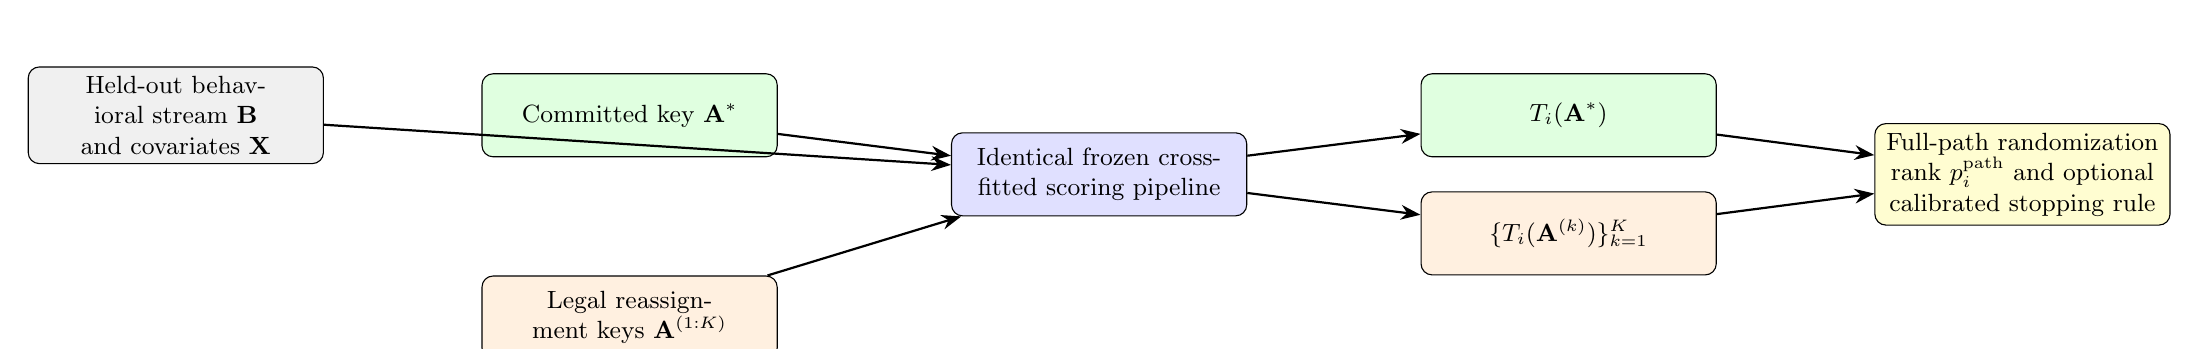
\begin{tikzpicture}[node distance=1.1cm, font=\scriptsize]
\node[bigblock, fill=gray!12] (data) {Held-out behavioral stream $\mathbf{B}$ and covariates $\mathbf{X}$};
\node[bigblock, fill=green!12, right=2.0cm of data] (true) {Committed key $\mathbf{A}^{*}$};
\node[bigblock, fill=orange!12, below=1.5cm of true] (controls) {Legal reassignment keys $\mathbf{A}^{(1:K)}$};
\node[bigblock, fill=blue!12, right=2.2cm of true, yshift=-0.75cm] (pipe) {Identical frozen cross-fitted scoring pipeline};
\node[bigblock, fill=green!12, right=2.2cm of pipe, yshift=0.75cm] (ttrue) {$T_i(\mathbf{A}^{*})$};
\node[bigblock, fill=orange!12, right=2.2cm of pipe, yshift=-0.75cm] (tnull) {$\{T_i(\mathbf{A}^{(k)})\}_{k=1}^{K}$};
\node[bigblock, fill=yellow!18, right=2.0cm of ttrue, yshift=-0.75cm] (rank) {Full-path randomization rank $p_i^{\mathrm{path}}$ and optional calibrated stopping rule};
\draw[arrow] (data) -- (pipe);
\draw[arrow] (true) -- (pipe);
\draw[arrow] (controls) -- (pipe);
\draw[arrow] (pipe) -- (ttrue);
\draw[arrow] (pipe) -- (tnull);
\draw[arrow] (ttrue) -- (rank);
\draw[arrow] (tnull) -- (rank);
\end{tikzpicture}%
}
\caption{Primary confirmatory inference. The identical frozen scoring pipeline is evaluated on the committed key and every legal reassignment key. The complete committed-key evidence path is ranked against the identically processed legal-key paths. A maximum-excursion path statistic includes all registered looks in the randomization reference distribution; any early stopping rule must also be calibrated across the full key-path ensemble.}
\label{fig:sequential}
\end{figure}

\subsection{Phase 3: Characterization After Validation}
\label{sec:phase3}

Protocol-specific validated candidates meeting the Phase 2 full-path randomization threshold undergo unsupervised characterization using hierarchical density-based clustering (HDBSCAN), with supervised models used only after preregistered labels exist (Section~\ref{sec:supervised}). Characterization is a profiling step applied after validation and contributes no validation evidence of its own.

Hierarchical density-based clustering identifies the geometric structure of candidate response-pattern deviations in the mixed-feature space, distinguishing dense clusters (shared candidate signatures) from sparse outliers (idiosyncratic patterns). The algorithm classifies each response vector as \textit{core} (within a dense cluster), \textit{border} (edge of cluster), or \textit{noise} (isolated outlier):

\begin{equation}
\text{HDBSCAN}(\mathbf{r}_i; \text{min\_cluster\_size}, \text{min\_samples}) \rightarrow \{C_1, C_2, \ldots, C_k, \text{Noise}\}
\label{eq:dbscan}
\end{equation}

with each extracted cluster assigned a persistence score over the density hierarchy,
\begin{equation}
\pi(C_k) = \int_{\lambda_{\min}}^{\lambda_{\max}} \mathbb{1}\big[C_k(\lambda)\ \text{persists}\big]\, d\lambda,
\label{eq:persistence}
\end{equation}
where $\lambda$ indexes the density level. HDBSCAN is preferred over flat DBSCAN because it evaluates cluster persistence across a hierarchy of density thresholds and therefore does not depend on a single global radius, which is brittle in the eleven-dimensional mixed-feature space where bounded information-theoretic features and unbounded structural distances scale differently. When feature scaling or mixed data types distort density estimates, the feature vector may first be embedded using a preregistered mixed-data method such as factor analysis of mixed data (FAMD) or a Gower-distance-compatible manifold representation; dimensional reduction is treated as an optional characterization aid rather than a source of validation evidence.

This characterization enables candidate subtyping: replicated target-dependent cases may exhibit distinct behavioral modalities, such as temporal prediction, spatial pattern detection, or causal inference, that may be relevant for future task matching or validation design.

\subsection{Feature Engineering}

Eleven candidate features may be extracted from each participant's multi-session response data. None is independently confirmatory merely because it is unusual. A preregistered subset may enter the single target-conditioned predictive endpoint of Eq.~\ref{eq:complik}; when it does, its complete selection and fitting procedure is repeated for every legal key. Features not frozen inside that endpoint are secondary or exploratory, while HDBSCAN and supervised classifiers are post-validation characterization tools.

\begin{table}[h]
\centering
\caption{Candidate features for target-conditioned modeling and post-validation characterization. No row is independently confirmatory; primary inference is the legal-key randomization rank of Eq.~\ref{eq:keyrank}. $^{\dagger}$F5 is an optional model-based summary, not a confirmatory endpoint. $^{\ddagger}$F6 (HDBSCAN density persistence) is a Phase-3 characterization feature computed only after validation and contributes no Phase-2 validation evidence (Sections~\ref{sec:phase3},~\ref{sec:supervised}). N1--N5 are noise-as-feature dimensions that detect structure in error.}
\label{tab:features}
\begin{tabular}{@{}cllll@{}}
\toprule
& \textbf{Feature} & \textbf{Measures} & \textbf{Computation} & \textbf{Range} \\
\midrule
F1 & Response Consistency & Cross-session stability & $\rho(\mathbf{r}^{(t)}, \mathbf{r}^{(t')})$ & $[-1, 1]$ \\
F2 & Cross-Session Entropy & Predictability & $H(\mathbf{r})$ & $[0, \log M]$ \\
F3 & Cluster Convergence & Membership stability & $\text{Stability}(i)$ & $[0, 1]$ \\
F4 & Mahalanobis Distance & Null centroid deviation & $d_M(\mathbf{r}_i, \boldsymbol{\mu}_0)$ & $[0, \infty)$ \\
F5$^{\dagger}$ & Optional Posterior & Model-based summary & $P(\theta_i = 1 \mid \mathbf{D})$ & $[0, 1]$ \\
F6$^{\ddagger}$ & Density Persistence & HDBSCAN cluster stability & $\pi_{\text{HDBSCAN}}(\mathbf{r}_i)$ & $[0, 1]$ \\
\midrule
N1 & Temporal Asymmetry & Pre-stimulus deviation & $A_i = \max_\tau I(R_t; S_{t+\tau})$ & $[0, \infty)$ \\
N2 & Target Directionality & Signed target coupling & $\delta_i(\mathbf{A})$ & $[-1/M, 1-1/M]$ \\
N3 & Context Variance & Exploratory load modulation & $V_i = \sigma^2_{\text{high}} / \sigma^2_{\text{low}}$ & $(0, \infty)$ \\
N4 & Cross-Task Coherence & Transfer signature & $\bar{\rho}_{\text{CCA}}$ across tasks & $[0, 1]$ \\
N5 & Heavy Tails & Exploratory tail structure & $\hat{\alpha}$ (stable index) & $(0, 2]$ \\
\bottomrule
\end{tabular}
\end{table}

% ============================================================
% 4. MATHEMATICAL FOUNDATIONS
% ============================================================
\section{Mathematical Foundations}

\subsection{Target-Conditioned Randomization Model}

\subsubsection{Primary Predictive-Improvement Statistic}
\label{sec:lr}
The primary statistic is the cumulative held-out log predictive improvement $T_{i,t}(\mathbf{A})$ of Eq.~\ref{eq:cumllr}. The null model predicts behavior from conventional covariates $\mathbf{X}$ only; the target-conditioned model additionally receives the candidate key label $A_{jt}$. Both models use the same preregistered architecture, regularization, and cross-fitting schedule for every key. Any target-relative feature is created only within $\hat p_1$ from the candidate key and the symmetrically represented option layout, then rebuilt from scratch for each legal reassignment key; the null branch is never supplied that information. A target-independent response style can improve neither the committed key uniquely nor its rank against exchangeable legal reassignments, even if that style is unusual, stable, or cluster-specific.

The fixed-horizon primary inference is the randomization rank of Eq.~\ref{eq:keyrank}. For a two-sided scientific question, sign is not created by taking an absolute final-answer deviation after inspection; rather, the target-conditioned model is specified in advance to admit both attraction and suppression, and the identical model is evaluated for every key. Secondary signed summaries, including $\delta_i$, distinguish attractor and suppressor profiles only after dependence is established.

\subsubsection{Sequential Calibration}
The cumulative statistic is not assumed to be an exact likelihood ratio, so Wald's analytic guarantees are not invoked. Type-I error and session boundaries are established by end-to-end null simulation and legal-key randomization under the complete registered pipeline. The calibration set must include realistic perseveration, alternation, fatigue, device drift, missing gaze samples, and participant-specific response biases. Operating characteristics are reported across a grid of injected target effects and must include familywise error across screened participants where population-scale use is contemplated.

\subsubsection{Prior Sensitivity and Optional Posterior}
\label{sec:prior}
The optional posterior in Eq.~\ref{eq:bayes} requires a prior on stable target dependence under the protocol. Three quantities must remain distinct:
\begin{itemize}[nosep]
\item $\pi_{\mathrm{population}}$: an assumed pre-screening prevalence used only in sensitivity analysis;
\item $q_{\mathrm{flag}}=P(\mathrm{flag})$: the observed marginal screening yield; and
\item $\pi_{\mathrm{screened}}=P(\theta_i=1\mid\mathrm{flag})$: the post-screening prior implied by an assumed prevalence and a model-based screening sensitivity.
\end{itemize}
The screening yield is not the screened prior. Formally,
\begin{equation}
\pi_{\mathrm{screened}}=
\frac{\pi_{\mathrm{population}}P(\mathrm{flag}\mid\theta_i=1)}{q_{\mathrm{flag}}}.
\label{eq:piscreened}
\end{equation}
Initially, $P(\mathrm{flag}\mid\theta_i=1)$ can come only from injected-signal simulations, preregistered positive controls, or later independently replicated cases. It cannot be estimated as an empirical anomaly sensitivity from an ordinary unlabeled calibration cohort. Posterior results must therefore be accompanied by a prior-sensitivity analysis and must not replace the design-based randomization result.

\subsection{Noise Dimension Formalizations}

The five noise dimensions introduced in Section~\ref{sec:naf} require formal mathematical treatment. Each dimension extracts a distinct form of structure from the error residuals defined in one-hot indicator space: a categorical response $r_{ij}^{(t)} \in \{1, \ldots, M\}$ is encoded as the indicator vector $\mathbf{o}_{ij}^{(t)} \in \{0,1\}^M$, and the residual is $\mathbf{e}_i^{(t)} = \mathbf{o}_i^{(t)} - \boldsymbol{\mu}_0$, where $\boldsymbol{\mu}_0 = (1/M, \ldots, 1/M)$ is the null expectation. Subtraction is defined on the indicators, not on the raw labels, which carry no metric.

\subsubsection{N1: Temporal Asymmetry , Anticipatory Mutual Information}

The most theoretically diagnostic discriminator is temporal asymmetry: the presence of response deviation that clusters \textit{before} external stimuli rather than after (Figure~\ref{fig:temporal}). This dimension requires a time-varying presented stimulus sequence $S_{t}$ and therefore applies only to task variants that present such a sequence, namely presentiment-style and embedded-task protocols; the canonical blank forced-choice task presents only a static hidden key and does not admit N1. For variants that do present a stimulus stream, define the anticipatory mutual information:

\begin{equation}
A_i(\tau) = I(R_t^{(i)}; S_{t+\tau}) = \sum_{r,s} p(r,s;\tau) \log \frac{p(r,s;\tau)}{p(r) \cdot p(s)}, \quad \tau > 0
\label{eq:ami}
\end{equation}

where $R_t^{(i)}$ is participant $i$'s response at trial $t$, $S_{t+\tau}$ is the stimulus presented $\tau$ trials later, and the joint distribution $p(r,s;\tau)$ is estimated empirically across trials. The scalar anticipatory feature is:

\begin{equation}
A_i = \max_{\tau \in [1, \tau_{\max}]} A_i(\tau)
\end{equation}

Under the null hypothesis (no anticipatory capability), $A_i(\tau) \to 0$ for all $\tau > 0$ as trial count increases. Significance is assessed via permutation testing: stimulus sequences are shuffled $B = 10{,}000$ times. Because $A_i$ is itself a maximum over the lag range $\tau \in [1, \tau_{\max}]$, each permutation recomputes the same maximum, $A_i^{*(b)} = \max_{\tau} A_i^{*(b)}(\tau)$, so that the null distribution $\{A_i^{*(b)}\}_{b=1}^{B}$ is the distribution of the \emph{maximized} statistic and the resulting $p$-value, $\hat{p} = |\{b : A_i^{*(b)} \geq A_i\}| / B$, correctly accounts for the multiple comparison across lags.

The critical distinction (Figure~\ref{fig:temporal}c) is that post-stimulus mutual information $I(R_t; S_{t-\tau})$ for $\tau > 0$ is explainable by memory, priming, and conventional cognitive processing. Pre-stimulus mutual information, if it survives controls for leakage, autocorrelation, stimulus-generation artifacts, and analytic flexibility, is the more diagnostic case. This makes N1 the most theoretically diagnostic feature: it would not be expected under ordinary cognitive mechanisms once conventional temporal, procedural, and analytic confounds are excluded \cite{mossbridge2012,radin2004}. The phenomenon has been reported in controlled laboratory settings \cite{bem2011}, though replication attempts have yielded mixed results \cite{galak2012}, a pattern compatible with, but not evidence for, the framework's expectation that such effects may be intermittent, context-sensitive, and detectable only through an iterative multi-session methodology rather than single-session designs.

% ============================================================
% FIGURE: Temporal Asymmetry Detection
% ============================================================
\begin{figure}[t]
\centering
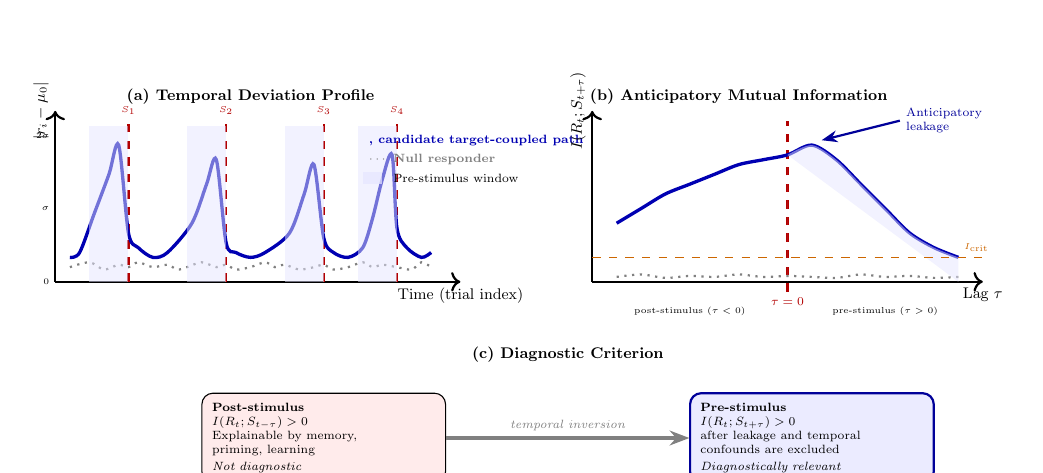
\begin{tikzpicture}[scale=0.62, every node/.style={transform shape}]

% === PANEL (a): Temporal deviation plot ===
\node[font=\small\bfseries] at (-6.5, 7.8) {(a) Temporal Deviation Profile};

\draw[thick,->] (-10.5, 4) -- (-2.2, 4) node[below, font=\small] {Time (trial index)};
\draw[thick,->] (-10.5, 4) -- (-10.5, 7.5) node[left, rotate=90, anchor=south, font=\small] {$|r_i - \mu_0|$};

\foreach \x in {-9, -7, -5, -3.5} {
    \draw[dashed, red!70!black, thick] (\x, 4) -- (\x, 7.3);
}
\node[above, font=\tiny, red!70!black] at (-9, 7.3) {$S_1$};
\node[above, font=\tiny, red!70!black] at (-7, 7.3) {$S_2$};
\node[above, font=\tiny, red!70!black] at (-5, 7.3) {$S_3$};
\node[above, font=\tiny, red!70!black] at (-3.5, 7.3) {$S_4$};

\draw[gray, thick, dotted] plot[smooth] coordinates {
    (-10.2,4.3) (-9.8,4.4) (-9.5,4.25) (-9.2,4.35) (-9,4.3)
    (-8.8,4.4) (-8.5,4.3) (-8.2,4.35) (-8,4.25) (-7.8,4.3)
    (-7.5,4.4) (-7.2,4.3) (-7,4.35) (-6.8,4.25) (-6.5,4.3)
    (-6.2,4.4) (-6,4.3) (-5.8,4.35) (-5.5,4.25) (-5.2,4.3)
    (-5,4.35) (-4.8,4.25) (-4.5,4.3) (-4.2,4.4) (-4,4.3)
    (-3.8,4.35) (-3.5,4.3) (-3.2,4.25) (-3,4.4) (-2.8,4.3)
};

\draw[blue!70!black, very thick] plot[smooth] coordinates {
    (-10.2,4.5) (-10,4.6) (-9.7,5.4) (-9.4,6.2) (-9.2,6.8) (-9,5.0)
    (-8.8,4.7) (-8.5,4.5) (-8.2,4.6) (-7.7,5.2) (-7.4,6.0) (-7.2,6.5) (-7,4.8)
    (-6.8,4.6) (-6.5,4.5) (-6.2,4.6) (-5.7,5.0) (-5.4,5.8) (-5.2,6.4) (-5,4.9)
    (-4.8,4.6) (-4.5,4.5) (-4.2,4.7) (-4.0,5.3) (-3.8,6.1) (-3.6,6.6) (-3.5,5.1)
    (-3.3,4.7) (-3,4.5) (-2.8,4.6)
};

\foreach \x in {-9, -7, -5, -3.5} {
    \fill[blue!10, opacity=0.5] (\x-0.8, 4) rectangle (\x, 7.2);
}

\node[right, font=\scriptsize, blue!70!black] at (-4.2, 6.9) {\textbf{, candidate target-coupled path}};
\node[right, font=\scriptsize, gray] at (-4.2, 6.5) {\textbf{$\cdots$ Null responder}};
\fill[blue!10, opacity=0.7] (-4.2, 6.0) rectangle (-3.8, 6.25);
\node[right, font=\scriptsize] at (-3.7, 6.12) {Pre-stimulus window};

\node[left, font=\tiny] at (-10.5, 4) {0};
\node[left, font=\tiny] at (-10.5, 5.5) {$\sigma$};
\node[left, font=\tiny] at (-10.5, 7) {$2\sigma$};

% === PANEL (b): Anticipatory Mutual Information ===
\node[font=\small\bfseries] at (3.5, 7.8) {(b) Anticipatory Mutual Information};

\draw[thick,->] (0.5, 4) -- (8.5, 4) node[below, font=\small] {Lag $\tau$};
\draw[thick,->] (0.5, 4) -- (0.5, 7.5) node[left, rotate=90, anchor=south, font=\small] {$I(R_t; S_{t+\tau})$};

\draw[red!70!black, thick, dashed] (4.5, 3.8) -- (4.5, 7.3);
\node[below, font=\scriptsize, red!70!black] at (4.5, 3.8) {$\tau = 0$};
\node[below, font=\tiny] at (2.5, 3.6) {post-stimulus ($\tau < 0$)};
\node[below, font=\tiny] at (6.5, 3.6) {pre-stimulus ($\tau > 0$)};

\draw[gray, thick, dotted] plot[smooth] coordinates {
    (1,4.1) (1.5,4.15) (2,4.08) (2.5,4.12) (3,4.1) (3.5,4.15) 
    (4,4.1) (4.5,4.12) (5,4.1) (5.5,4.08) (6,4.15) (6.5,4.1) 
    (7,4.12) (7.5,4.08) (8,4.1)
};

\draw[blue!70!black, very thick] plot[smooth] coordinates {
    (1,5.2) (1.5,5.5) (2,5.8) (2.5,6.0) (3,6.2) (3.5,6.4) 
    (4,6.5) (4.5,6.6) (5,6.8) (5.5,6.5) (6,6.0) (6.5,5.5) 
    (7,5.0) (7.5,4.7) (8,4.5)
};

\fill[blue!10, opacity=0.5] (4.5, 4) -- (4.5, 6.6) 
    plot[smooth] coordinates {(4.5,6.6) (5,6.8) (5.5,6.5) (6,6.0) (6.5,5.5) (7,5.0) (7.5,4.7) (8,4.5)}
    -- (8, 4) -- cycle;

\draw[dashed, orange!80!black] (0.5, 4.5) -- (8.5, 4.5);
\node[right, font=\tiny, orange!80!black] at (8.0, 4.7) {$I_{\text{crit}}$};

\draw[{Stealth[length=2mm]}-,thick, blue!60!black] (5.2, 6.9) -- (6.8, 7.3) 
    node[right, font=\scriptsize, text width=6em] {Anticipatory\\leakage};

% === PANEL (c): Key Distinction ===
\node[font=\small\bfseries] at (0, 2.5) {(c) Diagnostic Criterion};

\node[rectangle, draw, fill=red!8, text width=13em, rounded corners, 
      inner sep=6pt, font=\scriptsize] (post) at (-5, 0.8) {
    \textbf{Post-stimulus}\\$I(R_t; S_{t-\tau}) > 0$\\Explainable by memory,\\priming, learning\\[2pt]\textit{Not diagnostic}
};

\node[rectangle, draw=blue!60!black, fill=blue!8, text width=13em, rounded corners, 
      inner sep=6pt, font=\scriptsize, line width=0.8pt] (pre) at (5, 0.8) {
    \textbf{Pre-stimulus}\\$I(R_t; S_{t+\tau}) > 0$\\after leakage and temporal\\confounds are excluded\\[2pt]\textit{Diagnostically relevant}
};

\draw[-{Stealth[length=2.5mm]}, very thick, gray] (post.east) -- 
    node[above, font=\scriptsize\itshape] {temporal inversion} (pre.west);

\end{tikzpicture}
\caption{Temporal asymmetry detection. (a)~A candidate target-coupled path shows deviation spikes in pre-stimulus windows (blue shading), while null responders remain flat. (b)~Anticipatory mutual information peaks at positive lag ($\tau > 0$), indicating pre-stimulus structure (shaded). (c)~The diagnostic criterion: pre-stimulus correlation is diagnostically relevant only if it survives controls for leakage, autocorrelation, stimulus-generation artifacts, and analytic flexibility.}
\label{fig:temporal}
\end{figure}

\subsubsection{N2: Target-Relative Directionality}
A generic stable response bias is not evidence of target dependence. N2 is therefore defined relative to the candidate key, not as a nonzero mean residual in label space. The primary signed summary is the directional deviation
\begin{equation}
\delta_i(\mathbf{A})=\frac{1}{NT}\sum_{t,j}\mathbb{1}[r_{ijt}=A_{jt}]-\frac{1}{M},
\label{eq:n2target}
\end{equation}
with attraction indicated by $\delta_i>0$ and suppression by $\delta_i<0$. Its significance is not read from an asymptotic tail in isolation; the committed-key value is compared with the same statistic under legal reassignments. Transition-direction and gaze-direction summaries are treated analogously. N2 is secondary unless it is the preregistered sole primary endpoint or is frozen inside Eq.~\ref{eq:complik}.

\subsubsection{N3: Context-Modulated Variance}

If some component of the noise carries information, its statistical properties may respond to context. The framework models participant variance as a function of contextual load $C_t$ (cognitive difficulty, emotional arousal, environmental factors). The default specification is a random-effects structural variance model,
\begin{equation}
\sigma_i^2(C_t) = \omega_i + \beta_i \cdot C_t,
\label{eq:garch}
\end{equation}
in which variance scales with contextual load ($\beta_i \neq 0$) but no autoregressive term is fitted per subject. A fully autoregressive, GARCH-family specification with a lagged-variance term, $\gamma_i \cdot \sigma_i^2(C_{t-1})$, inspired by financial econometrics \cite{bollerslev1986}, is reserved for the large-sample regime: stable estimation of $(\omega, \beta, \gamma)$ requires far more sequential data than the five-session, few-hundred-trial individual record provides, and on short discrete categorical streams the optimization is prone to non-convergence and local minima. The autoregressive form is applied only to pooled or high-volume embedded data where the trial count justifies it, and the per-subject default omits the lag term. Unlike standard GARCH, the load term depends on an exogenous context variable rather than a lagged squared residual, reflecting the hypothesis that noise variance is modulated by experimental conditions rather than being self-exciting.

The operationalization of the contextual load variable $C_t$ is itself an open calibration problem: $C_t$ must be defined and validated in early pilot testing against independent physiological or task-difficulty markers, so that it captures genuine cognitive or affective shifts rather than introducing extraneous measurement noise into the variance model.

One proposed operationalization, suitable where computer-administered testing already records pointer telemetry, derives $C_t$ from motor kinematics rather than from any imposed task-difficulty parameter. With pointer coordinates sampled at $f_s \geq 60$\,Hz, instantaneous velocity is computed between successive samples, the acceleration profile $a_k$ is passed through a high-pass filter (for example a Butterworth filter above $10$\,Hz) to isolate micro-tremor from intentional ballistic movement, and $C_t$ is taken as the log-transformed variance of the filtered signal,
\begin{equation}
C_t = \log\!\left(\frac{1}{K}\sum_{k=1}^{K}\big(\mathcal{HPF}(a_k)\big)^2\right).
\label{eq:ctkinematic}
\end{equation}
To control for varying hardware polling rates and interface habituation across longitudinal sessions, the resulting series would be normalized per session by its median and median absolute deviation before entering the variance model of Eq.~\ref{eq:garch}. Because motor micro-variation may reflect hardware, posture, fatigue, or interface familiarity rather than cognitive load, $C_t$ must be validated against independent markers before being interpreted psychologically.

The noise feature is the conditional variance ratio:
\begin{equation}
V_i = \frac{\text{Var}(\mathbf{e}_i \mid C_t > C_{\text{median}})}{\text{Var}(\mathbf{e}_i \mid C_t \leq C_{\text{median}})}
\end{equation}

Context-modulated variance is common in ordinary human telemetry. N3 is therefore exploratory or characterizing unless a preregistered interaction between context and target-conditioned prediction is shown on held-out data and survives the legal-key randomization test.

\subsubsection{N4: Cross-Task Coherence}

If a participant's candidate anomaly signature reflects a stable underlying process rather than task-specific strategy, it may transfer across unrelated task domains. Given $K$ task types, the cross-task coherence for participant $i$ is measured via canonical correlation between anomaly signatures:
\begin{equation}
\rho_i = \frac{1}{\binom{K}{2}} \sum_{k < l} \text{CCA}_1(\mathbf{e}_i^{(k)}, \mathbf{e}_i^{(l)})
\end{equation}

where $\text{CCA}_1$ is the first canonical correlation coefficient between error vectors from tasks $k$ and $l$. Under the null hypothesis (independent noise across tasks), $\rho_i \to 0$. Replicated target-dependent cases may exhibit $\rho_i > 0$ across tasks whose surface features, target keys, and response formats are independently randomized; this is a characterization hypothesis, not independent confirmation. Because canonical correlation is unstable when the number of features approaches the number of observations, cross-task coherence is estimated only under a preregistered minimum trial count or with shrinkage or regularized CCA, and significance is assessed by task-label permutation.

\subsubsection{N5: Heavy-Tail Analysis}

Under many null models, aggregate residual statistics should approach thin-tailed behavior once the residual variable is properly specified. Candidate anomalies may produce heavy tails in specific preregistered variables, such as session-level deviations, inter-hit intervals, burst lengths, latency spikes, or target-coupled residuals. Where the measured residual variable is continuous or burst-like rather than bounded and categorical, the framework may fit $\alpha$-stable or alternative heavy-tail models \cite{nolan2020} to the residuals:
\begin{equation}
\hat{\alpha}_i = \arg\max_{\alpha \in (0, 2]} \mathcal{L}(\alpha \mid \{\mathbf{e}_i^{(t)}\}_{t=1}^{T})
\end{equation}

where $\alpha = 2$ corresponds to Gaussian and $\alpha < 2$ indicates heavy tails. The noise feature is $\hat{\alpha}_i$, with lower values indicating heavier tails. Significance is assessed by comparing $\hat{\alpha}_i$ against a preregistered cohort, bootstrap, or permutation-derived null distribution of tail indices. Tail-index estimates are treated as descriptive at the per-subject level unless the trial count is sufficient for stable estimation; otherwise heavy-tail evidence is evaluated by permutation or pooled calibration rather than by unconstrained $\alpha$-stable fitting.

\subsection{Information Leakage Model}

The noise-as-feature paradigm can be formalized through Shannon's information theory \cite{shannon1948,cover2006}. Each participant is modeled as a noisy channel between a hidden target state $S$ and an observable response $R$. The quantity of interest is the \textit{empirical mutual information}, or information leakage rate, between the source and the subject's responses, evaluated at the source distribution actually present in the experiment:
\begin{equation}
\hat{I}_i = I(S; R_i) = H(R_i) - H(R_i \mid S)
\label{eq:leakage}
\end{equation}

Empirical mutual information is upward-biased at small sample sizes: with a per-session trial count of order $N \approx 50$ to $250$, finite-sample fluctuations in the estimated joint distribution $\hat{p}(r,s)$ produce spurious positive $\hat{I}$ even for a true null responder, so that a naive estimator does not center at zero on short streams. The estimator is therefore bias-corrected. Writing $M$ for the number of response options and $M_S$ for the number of distinct target states, the Miller--Madow correction subtracts the leading-order bias term,
\begin{equation}
\hat{I}_i^{\text{corr}} = \hat{I}_i - \frac{(M-1)(M_S-1)}{2N \ln 2},
\label{eq:millermadow}
\end{equation}
and significance is assessed against a permutation null in which the target sequence is shuffled, so that residual bias is matched between the observed and null statistics rather than assumed away. Shrinkage estimators of the Panzeri--Treves family are an equivalent alternative where the alphabet is large relative to $N$.

Although the realized target vector is fixed after commitment, its target labels vary across trials, so empirical mutual information can be estimated from trial-level target--response pairs. The legal-key ensemble supplies inferential calibration. The measured quantity must not be confused with channel capacity. Channel capacity is the supremum of $I(S;R)$ over all source distributions, $C = \max_{p(S)} I(S;R)$, and computing it would require optimizing over hypothetical source distributions that the experiment does not realize; the framework makes no claim to the maximized quantity. The operationally relevant quantity is the leakage rate $\hat{I}_i$ at the source distribution the subject actually encounters.

For ideal null responders, $R_i$ is independent of $S$, so $\hat{I}_i \approx 0$. Candidate target dependence is described by $\hat{I}_i > 0$ with respect to the committed target state, but confirmation rests on the legal-key randomization rank of the complete pipeline. Both the attractor and the suppressor of Section~1.2 register as $\hat{I}_i > 0$: in the small-coupling regime the framework targets, a response stream reliably driven away from the target carries leakage comparable to one reliably drawn toward it, with the attainable avoidance signal bounded below the attainable attraction signal at large couplings for $M > 2$ (Section~\ref{sec:measurement}).

The variance paradox (Figure~\ref{fig:channel}) follows: a low-variance subject whose responses are statistically indistinguishable from uniform noise has $\hat{I}_i \approx 0$, regardless of how ``clean'' the data appears, while a subject whose deviations carry structure has $\hat{I}_i > 0$. The framework targets information leakage, structured deviation that carries mutual information with future or hidden states, rather than precision:

\begin{equation}
\text{Leakage}_i = \sum_{k=1}^{5} w_k \cdot N_k(i)
\end{equation}

where $N_k(i)$ are the five noise dimension scores and $w_k$ are weights that, in the current label-free protocol, are preregistered or estimated on the calibration cohort within the lockbox design of Section~\ref{sec:lockbox} rather than learned from a supervised classifier, since no validation labels exist prior to Phase~3. Where preregistered labels later become available, the weights may be re-estimated supervisedly as part of the optional Phase-3 characterization.

% ============================================================
% FIGURE: Information Leakage Channel Model
% ============================================================
\begin{figure}[t]
\centering
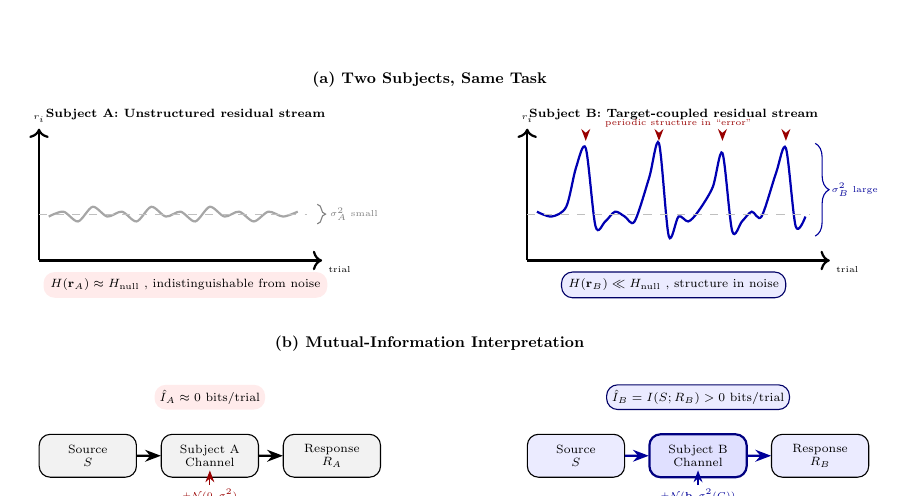
\begin{tikzpicture}[scale=0.62, every node/.style={transform shape}]

% === PANEL (a): Two variance profiles ===
\node[font=\small\bfseries] at (0, 8.2) {(a) Two Subjects, Same Task};

\node[font=\scriptsize\bfseries] at (-5, 7.5) {Subject A: Unstructured residual stream};
\draw[thick,->] (-8, 4.5) -- (-2.2, 4.5) node[below right, font=\tiny] {trial};
\draw[thick,->] (-8, 4.5) -- (-8, 7.2) node[above, font=\tiny] {$r_i$};
\draw[gray!70, thick] plot[smooth] coordinates {
    (-7.8,5.4) (-7.5,5.5) (-7.2,5.3) (-6.9,5.6) (-6.6,5.4) (-6.3,5.5) 
    (-6.0,5.3) (-5.7,5.6) (-5.4,5.4) (-5.1,5.5) (-4.8,5.3) (-4.5,5.6) 
    (-4.2,5.4) (-3.9,5.5) (-3.6,5.3) (-3.3,5.5) (-3.0,5.4) (-2.7,5.5)
};
\draw[dashed, gray!50] (-8, 5.45) -- (-2.5, 5.45);
\draw[decorate, decoration={brace, amplitude=3pt, mirror}, gray] 
    (-2.3, 5.25) -- (-2.3, 5.65) node[midway, right=4pt, font=\tiny] {$\sigma_A^2$ small};
\node[rectangle, fill=red!8, rounded corners, inner sep=4pt, font=\scriptsize] 
    at (-5, 4.0) {$H(\mathbf{r}_A) \approx H_{\text{null}}$ , indistinguishable from noise};

\node[font=\scriptsize\bfseries] at (5, 7.5) {Subject B: Target-coupled residual stream};
\draw[thick,->] (2, 4.5) -- (8.2, 4.5) node[below right, font=\tiny] {trial};
\draw[thick,->] (2, 4.5) -- (2, 7.2) node[above, font=\tiny] {$r_i$};
\draw[blue!70!black, thick] plot[smooth] coordinates {
    (2.2,5.5) (2.5,5.4) (2.8,5.6) (3.0,6.4) (3.2,6.8) (3.4,5.2) (3.6,5.3) 
    (3.8,5.5) (4.0,5.4) (4.2,5.3) (4.5,6.2) (4.7,6.9) (4.9,5.0) (5.1,5.4) 
    (5.3,5.3) (5.5,5.5) (5.8,6.0) (6.0,6.7) (6.2,5.1) (6.4,5.3) 
    (6.6,5.5) (6.8,5.4) (7.1,6.3) (7.3,6.8) (7.5,5.2) (7.7,5.4)
};
\draw[dashed, gray!50] (2, 5.45) -- (7.8, 5.45);
\draw[decorate, decoration={brace, amplitude=5pt, mirror}, blue!60!black] 
    (7.9, 5.0) -- (7.9, 6.9) node[midway, right=6pt, font=\tiny] {$\sigma_B^2$ large};
\foreach \x in {3.2, 4.7, 6.0, 7.3} {
    \draw[red!60!black, thick, -{Stealth[length=1.5mm]}] (\x, 7.1) -- (\x, 6.95);
}
\node[above, font=\tiny, red!60!black] at (5.1, 7.1) {periodic structure in ``error''};
\node[rectangle, fill=blue!8, rounded corners, inner sep=4pt, font=\scriptsize, 
      draw=blue!40!black, line width=0.4pt] 
    at (5, 4.0) {$H(\mathbf{r}_B) \ll H_{\text{null}}$ , structure in noise};

% === PANEL (b): Mutual information ===
\node[font=\small\bfseries] at (0, 2.8) {(b) Mutual-Information Interpretation};

\node[rectangle, draw, fill=gray!10, text width=5em, text centered, rounded corners,
      minimum height=2.5em, font=\scriptsize] (srcA) at (-7, 0.5) {Source\\$S$};
\node[rectangle, draw, fill=gray!10, text width=5em, text centered, rounded corners,
      minimum height=2.5em, font=\scriptsize] (chA) at (-4.5, 0.5) {Subject A\\Channel};
\node[rectangle, draw, fill=gray!10, text width=5em, text centered, rounded corners,
      minimum height=2.5em, font=\scriptsize] (outA) at (-2, 0.5) {Response\\$R_A$};
\draw[-{Stealth[length=2mm]}, thick] (srcA) -- (chA);
\draw[-{Stealth[length=2mm]}, thick] (chA) -- (outA);
\node[font=\tiny, red!60!black] at (-4.5, -0.3) {$+ \mathcal{N}(0, \sigma^2)$};
\draw[-{Stealth[length=1.5mm]}, red!60!black] (-4.5, -0.1) -- (-4.5, 0.2);
\node[rectangle, fill=red!8, rounded corners, inner sep=3pt, font=\scriptsize] 
    at (-4.5, 1.7) {$\hat{I}_A \approx 0$ bits/trial};

\node[rectangle, draw, fill=blue!8, text width=5em, text centered, rounded corners,
      minimum height=2.5em, font=\scriptsize] (srcB) at (3, 0.5) {Source\\$S$};
\node[rectangle, draw=blue!50!black, fill=blue!12, text width=5em, text centered, rounded corners,
      minimum height=2.5em, font=\scriptsize, line width=0.8pt] (chB) at (5.5, 0.5) {Subject B\\Channel};
\node[rectangle, draw, fill=blue!8, text width=5em, text centered, rounded corners,
      minimum height=2.5em, font=\scriptsize] (outB) at (8, 0.5) {Response\\$R_B$};
\draw[-{Stealth[length=2mm]}, thick, blue!60!black] (srcB) -- (chB);
\draw[-{Stealth[length=2mm]}, thick, blue!60!black] (chB) -- (outB);
\node[font=\tiny, blue!60!black] at (5.5, -0.3) {$+ \mathcal{N}(\mathbf{b}, \sigma^2(C))$};
\draw[-{Stealth[length=1.5mm]}, blue!60!black] (5.5, -0.1) -- (5.5, 0.2);
\node[rectangle, fill=blue!8, draw=blue!40!black, rounded corners, inner sep=3pt, 
      font=\scriptsize, line width=0.4pt] 
    at (5.5, 1.7) {$\hat{I}_B = I(S; R_B) > 0$ bits/trial};

\end{tikzpicture}
\caption{Information leakage channel model. (a)~Subject~A shows an unstructured residual stream indistinguishable from the matched null ($\hat{I}_A \approx 0$) despite low apparent variability, while Subject~B shows a target-coupled residual stream with structured dependence on the source ($\hat{I}_B > 0$). (b)~Mutual-information interpretation: Subject~B's residuals are biased and context-modulated, carrying nonzero mutual information with the source. The framework seeks target-coupled information leakage, not variance magnitude.}
\label{fig:channel}
\end{figure}

\subsection{Density-Based Clustering Parameterization}
\label{sec:dbscan}

HDBSCAN \cite{campello2013} is parameterized by a minimum cluster size and a minimum-samples value rather than a single global neighborhood radius, and it extracts clusters by their stability across a hierarchy of density levels. The parameters \texttt{min\_cluster\_size} and \texttt{min\_samples} are preregistered or sensitivity-tested on the calibration cohort, not tuned on validation outcomes.\footnote{For flat DBSCAN only, a global radius can be estimated from the knee of the $k$-distance curve, $\varepsilon^* = \arg\max_\varepsilon \left| \frac{d^2}{d\varepsilon^2} k\text{-dist}(\varepsilon) \right|$, with MinPts near $\dim(\mathbf{r}) + 1$ \cite{ester1996}; this is not part of the primary HDBSCAN characterization protocol and is noted only for comparison.}

Density-based clustering is applied only after transformation into the preregistered mixed-feature space, using Hamming or Gower dissimilarity for categorical components and calibrated continuous representations for behavioral telemetry, and it is not applied to raw categorical answer labels under a Euclidean metric, for which density notions are not well defined. In the eleven-dimensional mixed-feature space, a single global radius $\varepsilon$ is brittle, since bounded information-theoretic features and unbounded structural distances scale differently and inter-point distances become increasingly uniform as dimensionality grows. HDBSCAN is preferred over flat DBSCAN, because it selects clusters by their persistence across a hierarchy of density levels rather than by one global radius, which avoids the binary failure mode in which the procedure either collapses all subjects into a single core cluster or labels nearly every subject as noise. Where mixed feature scales distort density estimation, an optional dimension-reduction step (for example factor analysis of mixed data, or a Gower-distance-compatible embedding) may precede clustering; this remains an optional characterization aid and the framework's evidentiary core does not depend on it.

\subsection{Supervised Classification (Phase 3, Label-Conditional)}
\label{sec:supervised}
A supervised classifier requires labels that are external to the classifier. No such labels exist before the target-conditioned randomization test and independent replication. Supervised classification is therefore restricted to Phase~3 and contributes no Phase~2 evidence. The confirmatory pipeline terminates at the legal-key randomization result, accompanied by prespecified signed secondary summaries.

Once independently replicated cases and matched controls exist, a preregistered classifier such as gradient-boosted decision trees may be trained for behavioral subtyping or prediction of replication status:
\begin{equation}
\hat{\theta}_i = \operatorname{XGBoost}(\mathbf{f}_i)
=\sigma\!\left(\sum_{m=1}^{M}\eta h_m(\mathbf{f}_i)\right).
\end{equation}
Evaluation requires an untouched test cohort and must report calibration, discrimination, and decision-analytic utility. AUC alone is insufficient, and no classifier output retroactively strengthens the evidence that created its labels.

% ============================================================
% 5. IDENTIFICATION PROTOCOL
% ============================================================
\section{Identification Protocol}

Algorithm~\ref{alg:protocol} specifies the proposed target-dependence identification protocol.

\begin{algorithm}[t]
\caption{Persistent Target-Dependence Identification Protocol}
\label{alg:protocol}
\begin{algorithmic}[1]
\REQUIRE Cohort $\mathcal{C}$, registered legal-key assignment space, reassignment count $K$, session budget $T$, preregistered path functional $\Phi$, screening threshold $\tau_s$
\ENSURE Protocol-specific validated candidates and post-validation profiles
\STATE Partition $\mathcal{C}$ into disjoint discovery, calibration, and held-out validation cohorts
\STATE On discovery/calibration data, freeze preprocessing, key-independent conventional covariates $\mathbf{X}$, model class, cross-fitting folds, feature-selection rule, committed-secret key generator, $K$ chosen to resolve the adjusted error threshold, and path functional $\Phi$
\STATE \textbf{// Phase 1: screening only}
\STATE Estimate candidate behavioral phenotypes on discovery data; set $\tau_s$ on calibration data
\STATE Apply the frozen screen to validation subjects and form candidate set $\mathcal{F}$
\STATE \textbf{// Phase 2: target-conditioned confirmation}
\FOR{each $i\in\mathcal{F}$ and session $t=1,\ldots,T$}
    \STATE Compute $T_{i,t}(\mathbf{A}^{*})$ using the frozen cross-fitted pipeline
    \FOR{$k=1,\ldots,K$}
        \STATE Rerun the identical complete pipeline to compute $T_{i,t}(\mathbf{A}^{(k)})$
    \ENDFOR
\ENDFOR
\STATE Apply $\Phi$ to each complete key path and compute $p_i^{\mathrm{path}}$ by Eq.~\ref{eq:pathrank}
\STATE $\mathcal{V}\leftarrow\{i\in\mathcal{F}: p_i^{\mathrm{path}}\leq\alpha_{\mathrm{adj}}\}$
\STATE Label members of $\mathcal{V}$ as protocol-specific validated candidates, not persistent anomalies
\STATE Require an independent preregistered replication before applying the persistent designation
\STATE \textbf{// Phase 3: characterization only}
\STATE Apply HDBSCAN or supervised models to replicated cases and matched controls; contribute no Phase-2 evidence
\RETURN $\mathcal{V}$ with target-dependence statistics, signed secondary profiles, and replication status
\end{algorithmic}
\end{algorithm}

% ============================================================
% FIGURE 4: Comparison Table
% ============================================================
\begin{table}[t]
\centering
\caption{Comparison of historical and proposed identification methodologies}
\label{tab:comparison}
\begin{tabular}{@{}p{3.2cm}p{5.0cm}p{5.0cm}@{}}
\toprule
\textbf{Dimension} & \textbf{Stargate-Era Approach} & \textbf{Proposed Framework} \\
\midrule
Assessment Design & Structured tasks with known targets & Unstructured tasks with no external cues \\
Session Count & Single or limited sessions & Simulation-determined longitudinal budget; no universal minimum \\
Statistical Method & Frequentist hypothesis testing & Target-conditioned full-pipeline randomization inference; characterization after validation \\
Classification Criterion & $p$-value thresholds & Full-path legal-key randomization rank; optional stopping calibrated over key paths \\
False Positive Control & Limited (single-session) & Full-pipeline legal-key randomization, held-out lockbox, calibrated repeated-look control \\
Characterization & Subjective expert assessment & HDBSCAN subtyping + ML classification \\
Scalability & Manual, $O(1)$ experts & Automated, $O(N)$ cohort screening \\
\bottomrule
\end{tabular}
\end{table}

% ============================================================
% 6. ETHICAL FRAMEWORK
% ============================================================
\section{Ethical Framework}
\label{sec:ethics}

The identification of protocol-specific target dependence involves collection and analysis of sensitive cognitive and behavioral telemetry and therefore raises significant ethical considerations.

\subsection{Informed Consent}

Participants must be informed that the study concerns cognitive response patterns and hidden-target analysis, the nature of the tasks (unstructured response exercises), and the disposition of their data (pseudonymized storage, authorized access only), even if specific scoring details are withheld until debriefing. In contexts where full purpose disclosure would compromise the assessment, by enabling conscious strategy development that defeats the unstructured design, partial disclosure may be ethically permissible only under independent ethics review, provided that: (a) participants are informed that full debriefing will occur post-assessment; (b) no deception regarding personal risk or data use occurs; and (c) the protocol has been reviewed by an independent ethics committee.

\subsection{Data Protection}

Response data are pseudonymized at collection using random study identifiers. Direct identifiers are stored separately from response data in encrypted linkage files with access restricted to authorized research personnel. Where hashes are used, they are salted or keyed and are not treated as anonymization. Data retention follows the minimum necessary principle.

\subsection{Oversight and Accountability}

An independent review board evaluates all assessment protocols prior to implementation, monitors data handling practices, and adjudicates participant concerns. The review board includes representatives from ethics, law, cognitive science, and participant advocacy.

\subsection{Participant Welfare}

\begin{definition}[Non-Coercion Principle]
Target-dependence research must not result in coercion, exploitation, stigmatization, surveillance, or compulsory classification. Participants retain full autonomy regarding replication or follow-up, and no protocol-specific result creates an operational status or obligation.
\end{definition}

% ============================================================
% 7. APPLICATIONS
% ============================================================
\section{Applications}
Any application is contingent on independent replication, incremental validity over existing methods, calibration under the relevant base rate, net-benefit analysis, and domain-specific ethics review. The present framework supports a controlled concealed-target experiment; it does not yet justify personnel selection, clinical use, financial deployment, threat anticipation, or other operational classification. Its telemetry and randomization architecture may later be adapted to conventional prediction tasks, but usefulness in those domains must be demonstrated against external outcomes rather than inferred from competence-free target performance.

% ============================================================
% 8. DISCUSSION
% ============================================================
\section{Discussion}

\subsection{Addressing Historical Methodological Failures}

The framework addresses the methodological limitations summarized in Table~\ref{tab:comparison}: single-session assessment, absence of iterative validation, conflation of signal and noise, and lack of formal statistical criteria.

The framework departs from prior work in two respects. First, the noise-as-feature paradigm (Section~\ref{sec:naf}) inverts the standard analytical assumption: rather than treating response variability as error to be filtered, the framework analyzes five dimensions of structure within noise, formalized through Shannon's mutual-information framework. This addresses the fundamental problem that anomalous cognition, if it exists, may not present as a clean, stable signal but as structured deviation buried in stochastic processes. Second, the behavioral monitoring layer (Section~\ref{sec:behavioral}) is designed to recover pre-override structure that final-response-only analysis would miss. The override index (Eq.~\ref{eq:override}) captures a phenomenon invisible to final-response-only analysis: subjects whose initial selections or motor trajectories are target-coupled before later reversal. Together, analyzing structure in noise and recovering pre-override structure address a major limitation of Stargate-era designs, which measured only conscious performance on structured tasks.

\subsection{Generalization Beyond Anomalous Cognition}
\label{sec:generalization}
The concealed-target hypothesis can fail while parts of the measurement architecture remain useful. Multimodal behavioral telemetry, target-independent baseline modeling, cross-fitting, and full-pipeline randomization can be adapted to study ordinary intuition, forecasting, expert judgment, or subconscious decision processes. Such adaptation is not automatic: competence-free randomized targets contain no conventional predictive structure, so success or failure on them does not establish clinical, financial, or forecasting skill. Each conventional application requires an external criterion, incremental-validity testing, and a separate validation study.

\subsection{The Noise-as-Signal Principle}

The noise-as-feature move of Section~\ref{sec:naf} recurs across mature signal-detection disciplines. In gravitational-wave astronomy, the detection problem is the recovery of a structured waveform buried far below the instrumental noise floor, where the signal is recovered by correlation with a template at amplitudes the raw data would never reveal. In quantitative finance, persistent risk-adjusted excess return is distinguished from luck by the reproducibility of structure in a return stream across time. In fault detection and network intrusion analysis, the diagnostic signature is a statistical irregularity in otherwise noisy telemetry, identified against a learned baseline. The persistent anomaly framework imports the analytical standards of these fields, namely reproducibility, target specificity, and structure against a matched baseline, and applies them to human response streams. The contribution is the adaptation of these standards to a domain whose candidate signal is low-amplitude and distributed across the behavioral stream, and therefore systematically discarded by assessment paradigms built around single-session, final-answer scoring.

\subsection{Limitations}

\begin{enumerate}
    \item \textbf{Behavioral monitoring infrastructure.} The five-layer model (Table~\ref{tab:behavioral}) requires computer-administered protocols and, for gaze, device-specific calibration. Paper-based or low-bandwidth implementations lose attention, motor, and transition layers and reduce the framework to final-response analysis.
    \item \textbf{Threshold sensitivity.} The full-path randomization threshold and any optional stopping boundaries are calibrated for specificity and may miss individuals whose candidate signal is intermittent or context-sensitive.
    \item \textbf{Bootstrapping problem.} The ML classifier requires independently replicated target-dependent cases, creating a cold-start problem for initial deployment. The behavioral monitoring layer may partially mitigate this by providing richer per-subject feature vectors that may improve classifier performance at small sample sizes.
    \item \textbf{Override contamination.} The conscious override phenomenon (Eq.~\ref{eq:override}) could be confounded by general response uncertainty unrelated to intuitive signal. Distinguishing override-of-correct from general indecision requires sufficiently large item counts per session.
    \item \textbf{Finite-sample estimation choices.} At the target regime of $N \approx 50$ to $250$ trials per session, several estimators face known small-sample failure modes that the asymptotic forms do not capture, and the final choices belong to the preregistered statistical analysis plan rather than to the framework specification. The empirical mutual-information estimator can under-correct its bias when joint-bin occupancy is low, so significance must rest on a dependence-preserving surrogate null (for example a Markov or stationary-bootstrap surrogate that retains the subject's serial structure while severing target coupling) rather than on the corrected point estimate, with that estimate treated as descriptive below a minimum samples-per-bin ratio. The override transition baseline, if specified as a high-dimensional conditional probability over several covariates, is not estimable per subject at this trial count and must instead use a low-dimensional or penalized form (for example penalized splines on the covariates that require flexible form, with factors entered parametrically) selected by out-of-sample cross-validation on the subject's non-target items. The noise dimensions are mutually dependent; they are not multiplied as independent evidence. Unless frozen prospectively inside the single primary target-conditioned model and repeated for every legal key, they remain secondary or exploratory. These are estimation choices to be fixed against pilot data; the architecture does not depend on any single resolution, and the conservative options raise the per-subject session budget in a manner already consistent with the longitudinal, sequential accumulation model of Section~\ref{sec:sequential}.
    \item \textbf{No validation data yet.} The framework is theoretically grounded but requires empirical validation per the roadmap in Section~\ref{sec:roadmap}.
\end{enumerate}

% ============================================================
% 9. VALIDATION ROADMAP
% ============================================================
\section{Validation Roadmap}
\label{sec:roadmap}

% ============================================================
% FIGURE 6: Validation Roadmap
% ============================================================
\begin{figure}[t]
\centering
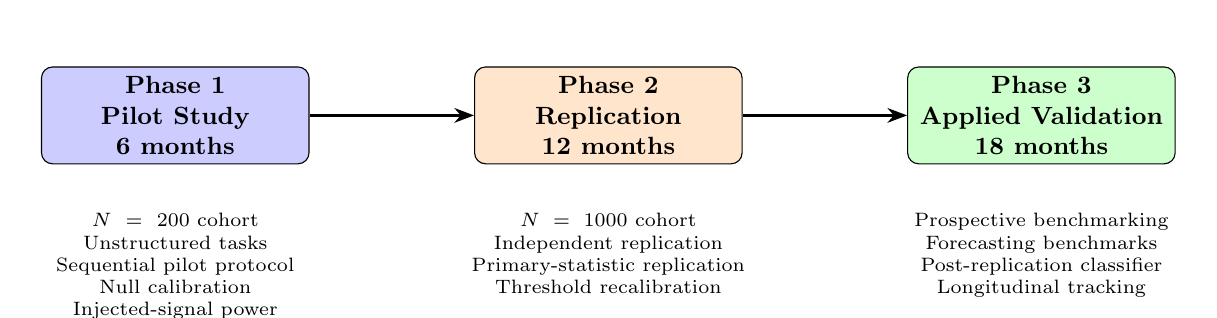
\begin{tikzpicture}[node distance=0.4cm]
    \node[phase, fill=blue!20, text width=9em] (p1) at (0,0) {Phase 1\\Pilot Study\\6 months};
    \node[phase, fill=orange!20, text width=9em] (p2) at (5.5,0) {Phase 2\\Replication\\12 months};
    \node[phase, fill=green!20, text width=9em] (p3) at (11,0) {Phase 3\\Applied Validation\\18 months};
    
    \draw[arrow] (p1) -- (p2);
    \draw[arrow] (p2) -- (p3);
    
    \node[below=0.5cm of p1, text width=10em, font=\scriptsize, align=center] {
        $N = 200$ cohort\\
        Unstructured tasks\\
        Sequential pilot protocol\\
        Null calibration\\Injected-signal power
    };
    \node[below=0.5cm of p2, text width=10em, font=\scriptsize, align=center] {
        $N = 1000$ cohort\\
        Independent replication\\
        Primary-statistic replication\\
        Threshold recalibration
    };
    \node[below=0.5cm of p3, text width=10em, font=\scriptsize, align=center] {
        Prospective benchmarking\\
        Forecasting benchmarks\\
        Post-replication classifier\\
        Longitudinal tracking
    };
\end{tikzpicture}
\caption{Three-phase validation roadmap from pilot testing through replication and applied validation.}
\label{fig:validation}
\end{figure}

\subsection{Acceptance Criteria}
\label{sec:acceptance}
Before any operational use, the framework must demonstrate:
\begin{enumerate}[nosep]
    \item \textbf{Null calibration:} end-to-end familywise or false-discovery-controlled error under legal-key full-path randomization, including every registered look and the number of screened participants; realistic simulated nulls supplement robustness and power analysis; a nominal per-subject target of $\alpha_{\mathrm{err}}\leq10^{-4}$ is used for large-scale screening unless a different value is justified prospectively. The legal-key ensemble or exact enumeration must have sufficient resolution for the smallest multiplicity-adjusted boundary, with $K\geq9{,}999$ required even to represent an unadjusted Monte Carlo rank of $10^{-4}$.
    \item \textbf{Sensitivity:} at least $0.90$ power for preregistered injected target-effect models at the smallest effect size the study claims to detect.
    \item \textbf{Positive predictive value:} reported across a conservative range of assumed population prevalences rather than inferred from specificity alone.
    \item \textbf{Independent replication:} the protocol-specific target-dependence result must reproduce in an independent preregistered cohort before a persistent designation is applied.
    \item \textbf{Incremental predictive validity:} any claimed conventional or applied capability must improve prediction of an external outcome beyond existing methods on held-out data.
    \item \textbf{Phase-3 classifier performance:} evaluated only after replicated labels exist, using an untouched test cohort and calibration as well as discrimination metrics.
\end{enumerate}

\subsection{Baseline Comparisons}

Phase 1 validation will compare the framework against two baselines:

\begin{enumerate}
    \item \textbf{Random selection:} Randomly designated ``anomalies'' assessed on identical forecasting tasks. Expected: no performance advantage.
    \item \textbf{Self-report:} Individuals self-identifying as possessing exceptional intuition. Hypothesis: marginal performance advantage, lower specificity than the framework.
\end{enumerate}

Any forecasting claim requires a separately powered, preregistered external-outcome study demonstrating incremental predictive validity over both baselines; concealed-target classification alone is insufficient.

% ============================================================
% 10. FUTURE WORK
% ============================================================
\section{Future Work}

Four primary research directions:

\begin{enumerate}
    \item \textbf{Neuroimaging studies.} fMRI and EEG examination of neural correlates of replicated target-dependence status. Any neuroimaging extension should be hypothesis-neutral and powered only after a reproducible behavioral phenotype exists; imaging is not used to validate the initial concealed-target result.
    \item \textbf{Longitudinal replication.} Multi-year testing of independently replicated target-dependent cases to assess stability, measurement drift, and protocol generalization.
    \item \textbf{External-outcome benchmarking.} Adapting the telemetry architecture to forecasting tasks and testing incremental validity against established baselines \cite{tetlock2015}.
    \item \textbf{Cross-domain adaptation.} Testing whether the methods generalize to separately validated decision tasks without assuming that competence-free target effects imply real-world skill.
\end{enumerate}

% ============================================================
% 11. ON THE NATURE AND ORIGIN OF THIS WORK
% ============================================================
\section{Declarations}

\subsection{What This Paper Contributes}

The contribution of this paper is a detection framework: a method for determining whether a human response stream carries reproducible, target-specific information about hidden or future targets, under controls designed to test whether a positive result survives bias, leakage, and analytic-flexibility explanations. The framework was developed through formalization, adversarial stress-testing, and consistency checks, with each hypothesis retained only where it could be converted into a falsifiable statistical test. The question of whether persistent anomalous cognition exists is one the framework is built to test rather than to assume.

\subsection{Disclosure of AI Tool Use}

Large language model systems (Claude, Anthropic; ChatGPT, OpenAI) were used substantively in preparing this manuscript, for mathematical formalization, equation derivation and dimensional checking, literature retrieval, citation organization, consistency checking, and prose preparation. The conceptual contributions originated with the author, who directed all uses of these tools, reviewed all claims and citations, and takes full and sole responsibility for the content of the manuscript and for its compliance with the policies of any venue to which it is submitted.

\subsection{Generality}

If the concealed-target hypothesis is false, components of the pipeline may still be adapted to conventional capacities as described in Section~\ref{sec:generalization}; such value requires separate external-outcome validation and is not guaranteed by the present task. The null hypothesis is explicit and the design is falsifiable; the next question is empirical.

% ============================================================
% 12. CONCLUSION
% ============================================================
\section{Conclusion}

This paper has presented an empirically testable framework for determining whether human response streams can exhibit persistent, target-specific deviations from chance expectation under committed-key, negative-control, and longitudinal validation conditions. By combining unstructured task design, target-conditioned full-pipeline randomization inference, sequential error control, and post-validation characterization, the framework reframes candidate exceptional intuition as a measurable response-stream hypothesis to be validated empirically.

The historical record demonstrates persistent institutional interest in anomalous cognitive capabilities across multiple decades and agencies. What has been lacking is not motivation but methodology. The framework proposed here addresses that gap directly, providing a statistical architecture for testing whether concealed-target dependence can be distinguished from target-independent behavior, characterizing the modality and magnitude of replicated effects, and, if validated, evaluating whether they have applied value in high-uncertainty contexts.

Whether persistent, target-specific structure of the kind described here can be reliably identified is an empirical question. The framework provides one testable measurement architecture with explicit controls and validation criteria.

\clearpage
\appendix

% ============================================================
% APPENDIX A: RETROCAUSAL TESTING
% ============================================================
\section{Retrocausal Testing via Historical Data Repositories}
\label{app:retro}

Claims of anomalous information transfer running counter to ordinary temporal order stand in the prior literature: the anticipatory-physiology meta-analyses report effects preceding their stimulus \cite{mossbridge2012}, the presentiment studies report retroactive influence on response \cite{bem2011}, and the SRI and Stargate-era programs claimed information transfer not reducible to conventional channels. This protocol does not assert that those claims are true. It supplies the instrument that would adjudicate them. If temporal nonlocality of the kind that literature asserts exists, then it must leave a detectable statistical signature in locked historical response data scored against a future-committed key; if it does not, that signature will be absent and the claim fails this test cleanly. The answer-pattern encoding methodology (Section~\ref{sec:ape}) makes this a falsifiable, first-principles prediction conditional on the prior claim, testable in either direction. Decades of standardized test responses, including the ASVAB, SAT, ACT, and state K--12 assessments, reside in institutional data repositories. Many such repositories may contain item-level response vectors, timestamps, scoring keys, and performance metadata at large scale.

The experimental protocol is:

\begin{enumerate}[nosep]
    \item Obtain a historical response dataset $\mathcal{D}_{\text{hist}}$ containing item-level responses from time $t_{\text{past}}$.
    \item At time $t_{\text{now}} > t_{\text{past}}$, generate a psi scoring key $\mathbf{A}^*_{\text{psi}}$ designating answer-pattern trials within the historical test structure.
    \item Score $\mathcal{D}_{\text{hist}}$ against $\mathbf{A}^*_{\text{psi}}$ using the pair-accuracy differential (Eq.~\ref{eq:pd}) assessed under the Markov-surrogate null.
    \item Compare observed pair accuracy against the null baseline computed from subjects' known item-level performance.
\end{enumerate}

Because the scoring key is generated after data collection but before analysis, under a precommitted key-derivation rule, the subjects were structurally isolated from any forward-causal exposure to it. Under a locked historical dataset, a public-beacon key, a precommitted mapping algorithm, blinded analysis, and a negative-control key set, above-chance pair accuracy on designated trials would not be attributable to direct forward-causal influence from the later-generated key itself, since the subjects could not have been influenced by a realized key value that did not yet exist. Such a result would, however, first require exhaustive examination for leakage, database artifacts, null-model failure, item-ordering and response-bias confounds, key-mapping bias, and analytic multiplicity before any nonstandard interpretation could be entertained.


\subsection{Experimental Controls}

The retrocausal design admits unusually strong controls that are difficult to implement in prospective psi experiments:

\textbf{Control 1: Exchangeable legal reassignment keys.} Generate a preregistered number $K$ of legal keys, each designating different subsets of item pairs and all derived from the same legal assignment space under Section~\ref{sec:committed-key}. The value of $K$ is set by the smallest adjusted significance level: $K=1{,}000$ is an illustrative exploratory setting with minimum rank $1/1001$, whereas a nominal $10^{-4}$ threshold requires at least $K=9{,}999$ before any sequential or population-level correction. Score $\mathcal{D}_{\text{hist}}$ against all $K$ keys. Under $H_0$ (no retrocausal effect), the distribution of key-specific pair accuracies should be consistent with the null baseline, up to sampling variation and dependence among overlapping item pairs. The primary key is fixed by the public-beacon commitment of Section~\ref{sec:committed-key}; no experimenter choice enters, and it cannot be selected, re-rolled, or adjusted after the data are seen. If the committed key produces elevated accuracy while the $K - 1$ control keys do not, the experiment gains $K - 1$ matched negative-control comparisons:

\begin{equation}
\text{Retrocausal Index} = \frac{\delta_{\text{designated}} - \mu(\{\delta_k\}_{k=1}^{K})}{\sigma(\{\delta_k\}_{k=1}^{K})}
\label{eq:retro}
\end{equation}

where $\delta_k$ is the pair accuracy deviation for key $k$. Because the $K$ control keys are mapped across a finite historical test structure, their designated subsets overlap and the deviations $\{\delta_k\}$ carry a dense covariance structure rather than being independent draws, so $\sigma(\{\delta_k\})$ misestimates the variance of an independent random key and the standard-normal assumption fails. The retrocausal index is retained only as a descriptive effect-size summary, and primary inference uses an exact non-parametric rank test of the committed key against the empirical control distribution,
\begin{equation}
p = \frac{1 + \sum_{k=1}^{K} \mathbb{1}\big(\delta_k \geq \delta_{\text{designated}}\big)}{K + 1},
\label{eq:retroperm}
\end{equation}
which requires no normality model and no mutual independence among key statistics. Its validity instead requires that the committed key be exchangeable under $H_0$ with the legal reassignment keys and that all keys be drawn from the same preregistered assignment space and scored by the identical complete pipeline.

\textbf{Control 2: Temporal-separation function.} Score datasets from progressively earlier time periods, $\mathcal{D}_{2024}$, $\mathcal{D}_{2020}$, $\mathcal{D}_{2015}$, $\mathcal{D}_{2005}$, against the same key generated at $t_{\text{now}}$. If a future-key dependence exists, its magnitude may vary as a function of temporal separation $\Delta t = t_{\text{now}} - t_{\text{past}}$:

\begin{equation}
\delta(\Delta t) = \delta_0 \cdot f(\Delta t)
\end{equation}

where $f(\Delta t)$ is the temporal-separation function. This analysis is exploratory unless one functional form or a complete model-comparison-and-selection procedure is preregistered and the selection maximum is included in the randomization calibration.

\textbf{Control 3: Frozen confound elimination.} Historical subjects cannot be affected by the later experimenter's expectations, demand characteristics, or sensory leakage associated with the future key, since they completed an assessment and departed long before any such key existed, and their responses are now frozen in a database. The remaining experimenter-controlled variables are dataset selection, preprocessing, key derivation, endpoint choice, and analysis decisions, which is why each must be precommitted under Section~\ref{sec:committed-key}.

\subsection{Connection to Nonlocality}

If the committed-key deviation is significant under the non-parametric rank test of Eq.~\ref{eq:retroperm}, such that historical behavioral output appears to carry mutual information with a future-generated scoring key, the result would constitute a physics-facing anomaly with potential implications for causal modeling, potentially testable with existing data subject to data access, privacy review, and analysis infrastructure, but only after leakage, database artifacts, null-model failure, item-order effects, and analytic flexibility had been excluded as sufficient explanations. Such a result would not demonstrate that the causal structure of the universe permits correlations across temporal separation; it would warrant that question, contingent on independent replication.

Answer-pattern encoding combined with committed-key controls makes this class of test possible, and historical repositories would provide a large-scale testbed without requiring new subject recruitment.

The null hypothesis can be specified explicitly: under $H_0$, pair accuracy on designated trials is governed by the subject-specific first-order transition model of Section~\ref{sec:ape} and does not depend on when the scoring key was generated. Pair accuracy on designated trials that exceeds this baseline in historical data scored against a future key would first indicate that the null model, the data pipeline, or the causal assumptions require scrutiny, and distinguishing among those possibilities would require the exhaustive elimination of leakage, artifacts, and analytic flexibility described above before any nonstandard interpretation could be entertained.


% ============================================================
% REFERENCES
% ============================================================
\begin{thebibliography}{99}

\bibitem{puthoff1976}
H.\,E. Puthoff and R. Targ, ``A perceptual channel for information transfer over kilometer distances: Historical perspective and recent research,'' \textit{Proceedings of the IEEE}, vol.~64, no.~3, pp.~329--354, 1976.

\bibitem{utts1996}
J. Utts, ``An assessment of the evidence for psychic functioning,'' \textit{Journal of Scientific Exploration}, vol.~10, no.~1, pp.~3--30, 1996.

\bibitem{smith2005}
P.\,H. Smith, \textit{Reading the Enemy's Mind: Inside Star Gate, America's Psychic Espionage Program}. Tom Doherty Associates, 2005.

\bibitem{air1995}
American Institutes for Research, ``An Evaluation of Remote Viewing: Research and Applications,'' Report prepared for the Central Intelligence Agency, 1995.

\bibitem{targ1977}
R. Targ and H.\,E. Puthoff, \textit{Mind-Reach: Scientists Look at Psychic Ability}. Delacorte Press, 1977.

\bibitem{mcmoneagle1997}
J. McMoneagle, \textit{Mind Trek: Exploring Consciousness, Time, and Space Through Remote Viewing}. Hampton Roads Publishing, 1997.

\bibitem{fama2010}
E.\,F. Fama and K.\,R. French, ``Luck versus skill in the cross-section of mutual fund returns,'' \textit{The Journal of Finance}, vol.~65, no.~5, pp.~1915--1947, 2010.

\bibitem{norman2017}
G.\,R. Norman \textit{et al.}, ``The causes of errors in clinical reasoning: Cognitive biases, knowledge deficits, and dual process theory,'' \textit{Academic Medicine}, vol.~92, no.~1, pp.~23--30, 2017.

\bibitem{busemeyer2012}
J.\,R. Busemeyer and P.\,D. Bruza, \textit{Quantum Models of Cognition and Decision}. Cambridge University Press, 2012.

\bibitem{pothos2013}
E.\,M. Pothos and J.\,R. Busemeyer, ``Can quantum probability provide a new direction for cognitive modeling?'' \textit{Behavioral and Brain Sciences}, vol.~36, no.~3, pp.~255--274, 2013.

\bibitem{ester1996}
M. Ester \textit{et al.}, ``A density-based algorithm for discovering clusters in large spatial databases with noise,'' in \textit{Proc.\ KDD-96}, pp.~226--231, 1996.

\bibitem{campello2013}
R.\,J.\,G.\,B. Campello, D. Moulavi, and J. Sander, ``Density-based clustering based on hierarchical density estimates,'' in \textit{Advances in Knowledge Discovery and Data Mining (PAKDD)}, Lecture Notes in Computer Science, vol.~7819, pp.~160--172, Springer, 2013.

\bibitem{wald1945}
A. Wald, ``Sequential tests of statistical hypotheses,'' \textit{Annals of Mathematical Statistics}, vol.~16, no.~2, pp.~117--186, 1945.

\bibitem{busemeyer2011}
J.\,R. Busemeyer \textit{et al.}, ``A quantum theoretical explanation for probability judgment errors,'' \textit{Psychological Review}, vol.~118, no.~2, pp.~193--218, 2011.

\bibitem{tetlock2015}
P.\,E. Tetlock and D. Gardner, \textit{Superforecasters: The Art and Science of Prediction}. Crown, 2015.


\bibitem{shannon1948}
C.\,E. Shannon, ``A mathematical theory of communication,'' \textit{The Bell System Technical Journal}, vol.~27, no.~3, pp.~379--423, 1948.

\bibitem{cover2006}
T.\,M. Cover and J.\,A. Thomas, \textit{Elements of Information Theory}, 2nd ed. Wiley-Interscience, 2006.

\bibitem{mossbridge2012}
J.\,A. Mossbridge, P. Tressoldi, and J. Utts, ``Predictive physiological anticipation preceding seemingly unpredictable stimuli: A meta-analysis,'' \textit{Frontiers in Psychology}, vol.~3, art.~390, 2012.

\bibitem{radin2004}
D.\,I. Radin, ``Electrodermal presentiments of future emotions,'' \textit{Journal of Scientific Exploration}, vol.~18, no.~2, pp.~253--273, 2004.

\bibitem{bollerslev1986}
T. Bollerslev, ``Generalized autoregressive conditional heteroskedasticity,'' \textit{Journal of Econometrics}, vol.~31, no.~3, pp.~307--327, 1986.

\bibitem{nolan2020}
J.\,P. Nolan, \textit{Stable Distributions: Models for Heavy Tailed Data}. Birkh\"{a}user, 2020.

\bibitem{bem2011}
D.\,J. Bem, ``Feeling the future: Experimental evidence for anomalous retroactive influences on cognition and affect,'' \textit{Journal of Personality and Social Psychology}, vol.~100, no.~3, pp.~407--425, 2011.

\bibitem{freeman2011}
J.\,B. Freeman and N. Ambady, ``MouseTracker: Software for studying real-time mental processing using a computer mouse-tracking method,'' \textit{Behavior Research Methods}, vol.~42, no.~1, pp.~226--241, 2010.

\bibitem{galak2012}
J. Galak \textit{et al.}, ``Correcting the past: Failures to replicate psi,'' \textit{Journal of Personality and Social Psychology}, vol.~103, no.~6, pp.~933--948, 2012.

\end{thebibliography}

\end{document}
